\documentclass{article}
\usepackage{graphicx}
\usepackage{wrapfig}
\usepackage{subcaption}
\usepackage[margin=1in]{geometry}
\usepackage{amsmath} % or simply amstext
\usepackage{amssymb}
\usepackage{siunitx}
\usepackage{booktabs}
\usepackage[export]{adjustbox}
\usepackage{cleveref}
\usepackage{booktabs}
\usepackage{gensymb}
\usepackage{float}
\usepackage[x11names,table]{xcolor}
\usepackage{setspace}
\usepackage[font=small]{caption}
\setstretch{1.5} % line spacing
\captionsetup[table]{font={stretch=1,small}} % line spacing in tables
\captionsetup[figure]{font={stretch=1,small}} % line spacing in figures
\usepackage{url}
% For timeline
\newcommand{\foo}{\color{LightSteelBlue3}\makebox[0pt]{\textbullet}\hskip-0.5pt\vrule width 1pt\hspace{\labelsep}}
\DeclareCaptionFont{blue}{\color{LightSteelBlue3}}
\usepackage{array,booktabs}
\usepackage[superscript,biblabel]{cite}  % make citations superscripts to save space
%\setlength{\belowcaptionskip}{-1.2\baselineskip}

\title{PhD Research Proposal: Molecular Level Design of Nanoporous Lyotropic Liquid
Crystal Membranes for Aqueous Separations \\ \vspace{0.5cm}
\large Advisors: Michael Shirts and Richard Noble}

\author{Benjamin J. Coscia} 

\begin{document}

  \graphicspath{{./figures/}}

  \maketitle
  \thispagestyle{empty}
  \clearpage
  \setcounter{page}{1} % don't count title page as a page 

  \section{State of the Art}\label{section:state-of-the-art}

  \subsection*{Commercial Membranes for Small Molecule Separations}
  
  % perhaps a word or two about micro and ultra filtration  
  
  %MRS: probably can do a little less introduction of the overall membrane needs, as we want to make sure 
  %MRS: the focus is on the research (thesis, you can include everything).  Can probably hold off that until you get the rest done, then trim as needed for space.
  %
  %MRS: remember the purpose of the introduction to any document is to lay out the rules of engagement; you want 
  %MRS: to raise the questions that the rest of the document will answer.
  % 
  %MRS: try to make sure the application motivation and the research described match up when possible.
  %MRS: if particular applications wouldn't be directly enabled by the research, at least draw to the connection
  %MRS: i.e. talk about the general tools of computation to understand nanostructured membranes, even if the current
  %MRS: membranes under development aren't suitable for the particular separations described.
  %BJC: Something like: The computational techniques developed here are suitable not just for LLC Membranes, but for any nanostructured 
  % membrane material.
  
    %MRS2: rephrase; sound like you are talking about only a minor problem. I would suggest adding a few more with citations
  %MRS2: to show you are aware of the breadth of the subject, and these aren't the only ones you know about.
  %represent a small subset
  %BJC2: rephrased then added 4 more citations
  
  More highly selective nanoporous membranes would be useful for 
  performing complex aqueous separations with seawater and various
  types of wastewater. For example, separating sodium chloride and 
  boron in seawater could yield potable drinking water in water scarce
  regions~\cite{fritzmann_state---art_2007} while separation of organic
  micropollutants found in municipal and industrial wastewaters could 
  make existing water supplies safer to drink~\cite{schwarzenbach_challenge_2006}.
  These represent only a few of the diverse contaminants of water sources~\cite{singh_production_2009,liu_removal_2008}. 
  By efficiently separating contaminants from feed solutions with
  highly selective membranes, it is possible to reduce the number of 
  required membrane passes and post-treatment steps needed for a given 
  filtration process \cite{werber_materials_2016}, thus lowering energy 
  requirements and cost. Additionally, one can extract valuable 
  resources from the feed streams~\cite{sales_resource_2015}. For example,
  flowback water produced during hydraulic fracturing of shale 
  formations contains dissolved species like acetate whose extraction has 
  economic value \cite{dischinger_application_2017,theodori_hydraulic_2014}.

  Reverse osmosis (RO) and nanofiltration (NF) are two prevailing commercial membrane
  filtration processes that can be used to separate solutes on the order of
  1 nm in size and smaller, including ions. Both apply hydraulic pressure 
  to the feed solution in order to overcome osmotic pressure and force water
  and unfiltered components through the membrane. RO membranes are typically
  thin film composite with a porous mechanical support layer and a thin but
  dense polymer matrix active layer where separations occur.\cite{jeong_interfacial_2007}
  RO separates solutes based on the solute's ability to dissolve into and 
  diffuse through the tortuous pathways available in the membrane's dense 
  active layer. RO offers high selectivity at the cost of relatively high 
  energy requirements since one must apply hydraulic pressure on the order of
  50--100 bar to the feed solution in order to achieve an economical flux~\cite{van_der_bruggen_review_2003}.
  In contrast to RO membranes, NF membranes have explicit pores on the order
  of 1 nm in size. Typically, separations are achieved based on size exclusion
  and Donnan exclusion if the membrane's surface has a net charge.~\cite{donnan_theory_1995}
  NF membranes require significantly less applied pressure in order to achieve solute flux
  comparable to RO. Unfortunately, conventional NF membrane synthesis processes, such as 
  phase-inversion\cite{smolders_microstructures_1992}, are stochastic in
  nature which yields pores that are polydisperse in size.\cite{werber_materials_2016}
  Pore size polydispersity is detrimental to membrane selectivity.
  
  The downfall of RO and NF membranes can be summarized by the well-known
  permeability-selectivity tradeoff. Namely, it is difficult to increase the
  permeability of a desired molecular or atomic species, while maintaining
  the same retention of undesired species.\cite{werber_materials_2016}  
  
  \subsection*{Nanostructured Membranes}
  
  % BJC2: condensed this section into one paragraph
  Nanostructured membranes attempt to overcome the permeability-selectivity 
  tradeoff through intelligent design at the molecular level. 
%  Graphene sheets, carbon nanotubes (CNTs) and zeolites are three highly
%  studied nanostructured technologies. 
  Ultrathin-film graphene and graphene oxide membranes are an active area
  of research because they are atomically thick and therefore offer potential
  for extremely high permeability membranes.~\cite{humplik_nanostructured_2011}
  However, scalable synthesis without introducing microscopic, performance
  degrading defects has not yet been achieved.~\cite{cohen-tanugi_multilayer_2016,wei_multilayered_2018}
  Carbon nanotubes (CNTs) have shown promise as aqueous separations membranes
  due to unprecedentedly fast water transport.\cite{humplik_nanostructured_2011,hummer_water_2001} 
  Practically, dispersing and aligning CNTs into a polymer matrix is extremely
  difficult because they tend to agglomerate due to Van der Waals forces.~\cite{sahoo_polymer_2010}
  Finally, zeolite-coated ceramic membranes offer the potential for permeabilities
  comparable to ultrafiltration, molecular sieves with pores up to 100 nm in 
  size~\cite{werber_materials_2016}, with selectivities as good as NF and RO. 
  A number of studies have tested the permeability and sodium salt rejection
  of various zeolite membranes, however none have fully overcome the 
  permeability-selectivity tradeoff.~\cite{pendergast_review_2011,auerbach_handbook_2003,li_novel_2007}


  %MRS2: this section is not so useful, becaue it talks about things you are NOT doing.  In a dissertation, would be good 
  %MRS2: context, but here, it distracts a bit because it's not summarizing what you are presenting in this paper. i.e. with 15 pages, you don't want to spend space talking about what you aren't doing.  Ideally, cut down to 1 paragraph just to
  %MRS2: show that you are aware of existing technologies.
  %BJC2: condensed above
%  Ultrathin-film graphene and graphene oxide membranes are a very active
%  area of research because they offer potential for extremely high 
%  permeability membranes. An ideal graphene membrane is a 2D material 
%  composed of a single layer of graphene.\cite{humplik_nanostructured_2011}
%  Synthesis of a single layer of graphene at a large scale without introducing
%  defects is a challenge that has not yet been overcome. Multilayered graphene
%  membranes are potentially easier to synthesize and more scalable which has 
%  resulted in an increasing interest over recent years.\cite{cohen-tanugi_multilayer_2016,wei_multilayered_2018}
%  
%  Carbon nanotubes (CNTs) have shown promise as aqueous separations membranes
%  due to unprecedentedly fast water transport.\cite{humplik_nanostructured_2011,hummer_water_2001} 
%  Practically, dispersing CNTs into a polymer matrix is extremely difficult
%  because they tend to agglomerate due to Van der Waals forces. Functionalization
%  of the CNT walls has been heavily investigated  as a way to overcome this issue, however 
%  alignment of the CNTs into an array feasible as a nanoporous membrane 
%  persists as a challenge to CNT membranes.\cite{sahoo_polymer_2010}
%   
%  
%  Zeolites have highly uniform nm-sized crystalline structures with cage-like
%  cavities that allow movement and trapping of small solutes. The crystalline
%  frameworks are typically formed by networks of silicon and aluminum each 
%  attached to 4 oxygen atoms in a tetrahedral arrangement.~\cite{auerbach_handbook_2003}
%  One can replace the silicon and aluminum atoms via ion exchange in order to
%  control the size of the cavities and hence its molecular-seiving properties.~\cite{li_novel_2007}
%  A number of studies have tested the permeability and sodium salt rejection
%  of various zeolite membranes, however none have fully overcome the 
%  permeability-selectivity tradeoff.~\cite{pendergast_review_2011}
%%    \item Most are prone to defects in the crystalline structure.

  \subsection*{Lyotropic Liquid Crystal Membranes}
  
  Preliminary evidence has shown that cross-linked lyotropic liquid crystal
  (LLC) membranes can be produced at moderate scale and may be capable of 
  performing highly selective separations~\cite{zhou_supported_2005,zhou_new_2007}. 
  LLCs are amphiphilic molecules that have the ability to self-assemble into
  porous nanostructures~\cite{smith_ordered_1997} that can be cross-linked 
  to create mechanically strong membrane films with periodic uniform-sized
  pores on the order of 1 nm in diameter~\cite{zhou_supported_2005}. 
  Since LLC polymer membranes have a very narrow pore size distribution, they 
  inherently exhibit high selectivity due to their molecular weight cut-off 
  (MWCO)~\cite{zhou_supported_2005}. Additionally, LLC monomers can be salts,
  and therefore lead to Donnan exclusion of ions at the membrane-feed solution 
  interface.\cite{donnan_theory_1995}
%    The membrane gains a net surface charge when counterions from
%  the head groups that line the pore walls escape into the feed solution in an
%  effort to balance the gradients of concentration and electric potential
%  \cite{donnan_theory_1995}.

  The feasibility of nanostructured LLC polymer membranes for selective separations
  has been demonstrated using LLC monomers that form the type 1 bicontinuous cubic
  (Q\textsubscript{I})~\cite{hatakeyama_water_2011,hatakeyama_nanoporous_2010,carter_glycerol-based_2012}
  and the inverted hexagonal (H\textsubscript{II}) 
  phases (see Figure~\ref{fig:structures}).~\cite{zhou_supported_2005} When separating organic solutes from NaCl, Q\textsubscript{I}-phase
  membrane filtration experiments have shown selectivity 2--3 times higher than
  commercial RO and 6--12 times higher than commercial NF membranes.~\cite{dischinger_application_2017}
  When separating a series of various sized dyes, an H\textsubscript{II}-phase 
  LLC membrane showed complete rejection of dyes bigger than 1.2 nm in size~\cite{zhou_supported_2005}.

%  \begin{wrapfigure}{L}{0.5\textwidth}
%  \centering
%  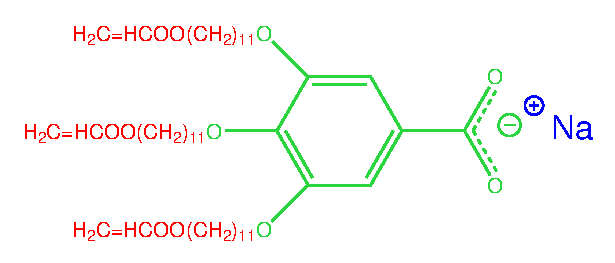
\includegraphics[width=\linewidth]{NaGA3C11_colorcoded.eps}
%  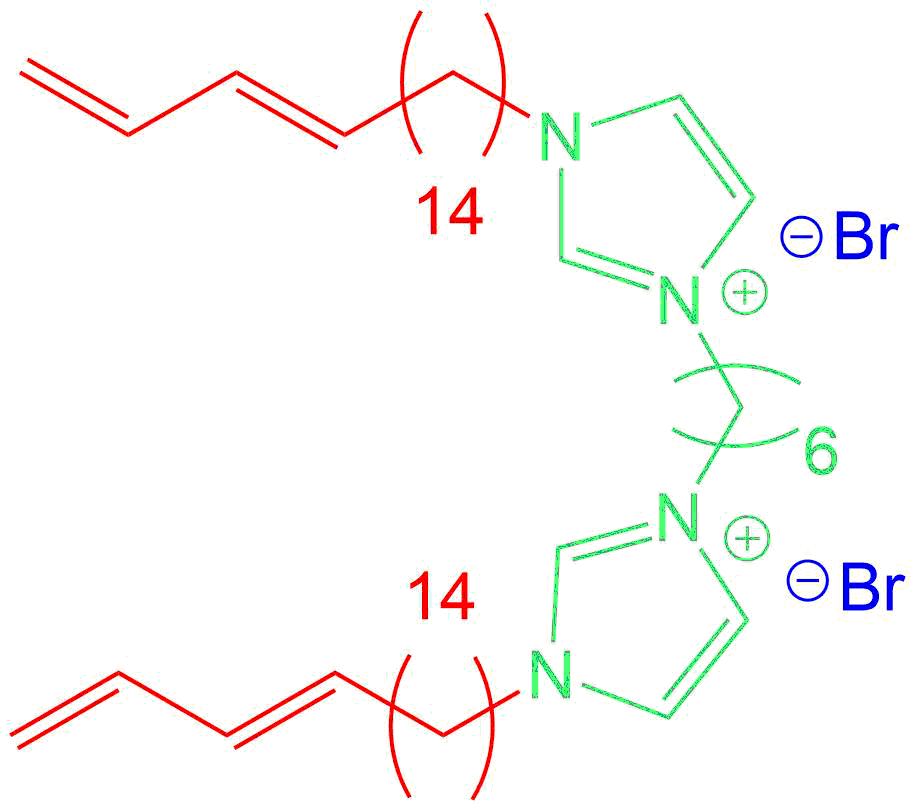
\includegraphics[width=0.8\linewidth]{q1_monomer.png}
%  \end{wrapfigure}

%  \begin{wrapfigure}{L}{0.75\textwidth}
  \begin{figure}
  \centering
  \begin{subfigure}{0.55\linewidth}
  \hspace{0.5cm}
  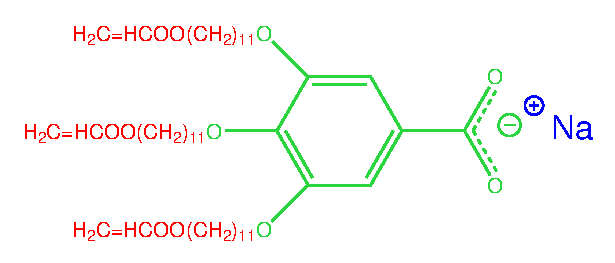
\includegraphics[width=0.8\linewidth]{NaGA3C11_colorcoded.eps}
  \vspace{1.4cm}
  \caption{}\label{fig:HII_mon}
  \end{subfigure}
  \begin{subfigure}{0.4\linewidth}
  \hspace{0.4cm}
  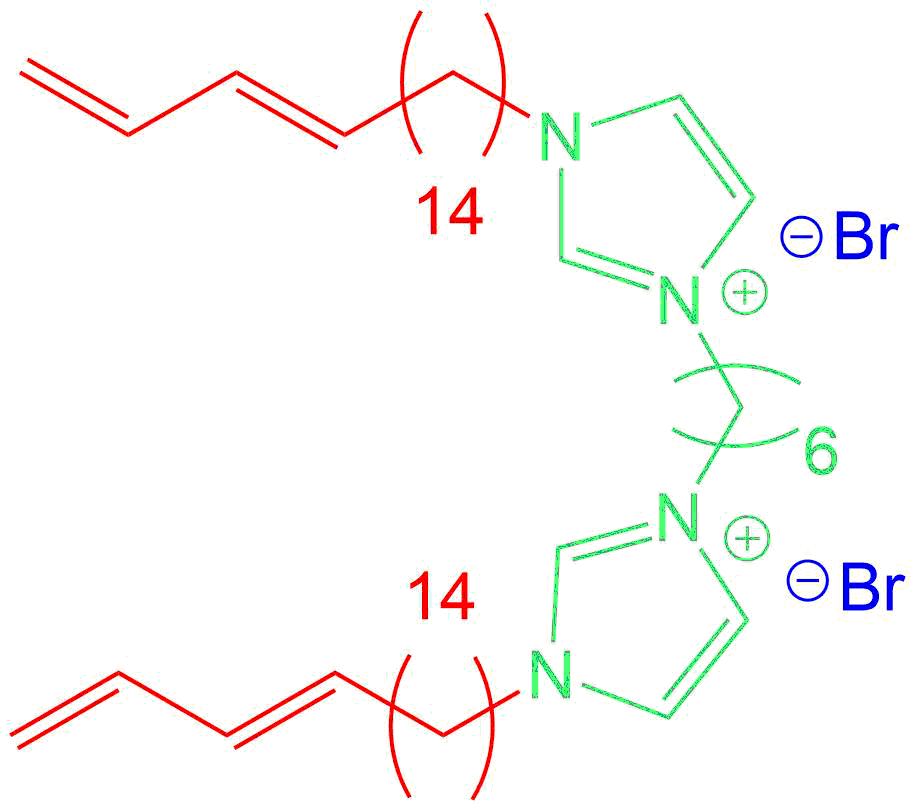
\includegraphics[width=0.7\linewidth]{q1_monomer.png}
  \caption{}\label{fig:q1_mon}
  \end{subfigure}
  \caption{H\textsubscript{II} and Q\textsubscript{I} phase LLC membranes have 
  been synthesized from monomers in (a) and (b) respectively. One can 
  alter membrane properties by modifying the length and number of tails (red), the
  functional head group (green) and the counterion identity (blue) of LLC monomers.}\label{fig:structures}
  \end{figure}

  Q\textsubscript{I}-phase membranes consist of a tortuous network of three
  dimensionally interconnected pores that prevent optimal through-plane
  transport. In contrast, the densely packed, non-tortuous and uniform sized
  pores of H\textsubscript{II}-phase membranes represent the ideal geometry
  for achieving high solute flux\cite{matyka_tortuosity-porosity_2008}. However,
  the hexagonally packed LC domains of the H\textsubscript{II}-phase are generally
  unaligned, which hurts membrane permeability. This domain scale misalignment
  had inhibited further development of this technology, and research efforts were
  focused on the Q\textsubscript{I} phase, whose geometry does not require 
  alignment~\cite{zhou_new_2007}.

%  The H\textsubscript{II}-phase pore geometry (Figure~\ref{fig:assembly}) has a
%  high theoretical capacity for transport than the Q\textsubscript{I} phase.
%  \begin{itemize}
%	  \item The H\textsubscript{II} phase forms at room temperature in the 
%	  presence of ca.~10 wt\% water and consists of hexagonally packed, 
%	  hydrophilic pore columns\cite{smith_ordered_1997}. 
%%	  \item The hexagonal, straight-pore geometry provides a dense array
%%	  of hydrophilic channels and short pathways for solutes to travel.
%	  % BJC: should rethink the following since we think that thermotropic doesn't exist
%	  \item In the absence of water, neat monomer will form the same hexagonal
%	  columnar structure which, in the literature, has been referred to as the
%	  Col\textsubscript{h} thermotropic phase\cite{feng_scalable_2014}.
%  \end{itemize}

  Recently, researchers learned how to macroscopically align the hexagonal 
  domains which has revived research into H\textsubscript{II}-phase LLC
  polymer membranes. In 2014, Feng et al.~showed that one can align Col\textsubscript{h}
  domains, a temperature-dependent hexagonal phase created by neat LLC monomers,
  using a magnetic field with subsequent cross-linking to lock the structure 
  in place\cite{feng_scalable_2014}. In 2016, Feng et al.~showed that one could 
  also obtain the same result by confining the neat monomer between PDMS or glass 
  substrates since hexagonal mesophases preferentially anchor perpendicular to 
  both surfaces\cite{feng_thin_2016}.
  
  Unfortunately, reproducing the work of Feng et al. with the hydrated 
  H\textsubscript{II} phase has been an experimental challenge. Therefore, the
  primary focus of experimental research efforts has been with the Q\textsubscript{I} 
  phase.

  \section{Project Objectives}\label{section:objectives}  
  
  Our current understanding of the molecular details of LLC membranes'
  nanostructure is not sufficient to be able to precisely design them for
  specific separations. Dischinger et al.~attempted to use an empirical model
  that correlates the physicochemical properties of the counterion used in
  a Q\textsubscript{I}-phase LLC membrane to solute rejection. Although there
  was some agreement with their empirical model, it does not offer a 
  sufficiently detailed explanation of the critical molecular interactions 
  leading to the observed behavior.~\cite{dischinger_effect_2017} 
  H\textsubscript{II}-phase LLC polymer membrane studies have been limited
  primarily to the Na-GA3C11 monomer (Figure~\ref{fig:HII_mon}) with
  some characterization done after minor monomer structural modifications. 
  These studies emphasized large scale structural features such as pore spacing
  as well as size-based rejection.~\cite{zhou_supported_2005,resel_structural_2000}
  Given the similar topology of H\textsubscript{II} and Q\textsubscript{I}
  membrane pores, we expect the H\textsubscript{II} phase will also be 
  subject to complex solute-membrane interactions that are not easily explained
  by an empirical model.

  A molecular-level understanding of structure and transport in LLC polymer 
  membranes, enabled by molecular dynamics (MD) simulations, can provide 
  guidelines to reduce the large chemical space available to design
  monomers for creation of separation-specific membranes. Using a sufficiently
  accurate molecular model, we can observe transport of solutes within LLC 
  membrane nanopores with atomistic resolution and infer mechanisms. 
  Based on this information we will have a much greater capability to 
  intelligently design new membranes by screening new liquid crystal monomer
  designs with MD simulations. The principles learned can be implemented 
  and tested experimentally.
  
  \noindent There are four primary objectives of this PhD research which are 
  at various stages of completion.

  \begin{enumerate}
  
    \item Develop techniques to build and understand the nanoscopic structure
    of LLC membranes. (\textcolor{green!40!olive}{\textbf{Complete}})

    %MRS2: Objectives shouldn't include a description of what has and hasn't 
    %been done.  Then it's not an really just an objective anymore. I would 
    %suggest rephrasing these in terms of the intellectual objective, focusing
    %on the questions to be asked and hypotheses to be tested, and then talk 
    %in the next section about what has been done (or is to do).
    %BJC2: got it, rephrased first 2 objectives.

    A useful molecular-level model should incorporate a detailed picture 
    of the nanoscopic pore structure, which is crucial to understanding
    the role of monomer structure in solute transport and membrane design.
    Therefore, we must first create an atomistic model that is maximally 
    consistent with experimental structural data. It is also necessary to
    evaluate and justify the minimum effort required to build systems with
    alternate monomers while maintaining an experimentally-consistent 
    chemical environment. 
    
%    I have created a maximally consistent structural model by comparing 
%    simulated X-ray diffraction (XRD) patterns, generated from MD trajectories,
%    to an experimental 2D wide angle X-ray scattering (WAXS) spectrum of a 
%    Col\textsubscript{h} phase LLC membrane. I have used this model as an 
%    example in order to 
%    %MRS2: I don't know that it's easy yet . . . 
%    %understand the ease with which 
%    demonstrate how 
%    we can apply our approach
%    to alternate monomers and other LC phases. 


%    shown that we achieve a
%    similar pore composition regardless of initial configuration which is 
%    influenced by a number of variables. This implies that our model can
%    
%        We will assess the extent to which
%    we can apply our understanding to the H\textsubscript{II} phase, as well
%    as systems built with alternate monomers.
    
    \item Determine solute-membrane interactions that give rise to
    transport mechanisms. (\textcolor{green!40!olive}{\textbf{Complete}})
    
    Using my most experimentally consistent configuration, I can place 
    small molecules within the H\textsubscript{II} nanopores and observe
    their behavior over simulation-accessible timescales. This objective 
    aims to organize observations of various solute behaviors into
    distinct mechanisms that can help guide membrane design based on 
    chemical functionality of both solutes and LLC monomers.
    
%    I observed the transport of a relatively large set of small polar solutes
%    placed within the H\textsubscript{II} phase membrane nanopores. I analyzed
%    the time series of each solute's position in addition to directly measuring
%    the physical interactions, such as hydrogen bonding and ion coordination, 
%    between solutes and LLC monomers.
    
    \item Create a stochastic model which can project long timescale 
    transport behavior. (\textcolor{blue}{\textbf{In Progress}})
    
    I will combine my qualitative knowledge of the solute transport mechanisms
    with simulation data in order to inform a stochastic model. This model
    should closely reproduce the properties of the time series that we observe 
    in our simulations. Due to the low computational cost of a stochastic model
    relative to MD simulations, I will be able to forecast long timescale transport
    behavior and make well-converged predictions of macroscopic transport properties.
           
    \item Adapt the same analysis to the Q\textsubscript{I} phase. (\textcolor{blue}{\textbf{In Progress}})
    
    Over the course of this project, experimental research surrounding
    LLC membranes has shifted nearly all focus towards the Q\textsubscript{I}
    phase due to its more facile synthesis.	Although most of my work has 
    been applied to the H\textsubscript{II} phase, much of the same analyses
    can be applied to the Q\textsubscript{I} phase. The biggest challenge will
    be adapting my techniques to its more complex three dimensional geometry.
    
%    \item Enable easy continuation of our work with a dedicated and 
%    well-documented python package.
%    
%	Although molecular simulations have become popular
%	for studying systems at the atomic level, LLCs used in this context
%	have not been heavily investigated. Consequently, much of the 
%	analysis developed for this project is not widely applied. Therefore, 
%	it is important for us to make available the scripts that reproduce
%	the exact results presented in our published papers along with detailed
%	documentation of the scripts. This will ensure near-seamless continuation
%	of this project and accelerate the development of LLC membranes.
    
  \end{enumerate}

  \section{Progress to Date}\label{section:progress}
  
  \textbf{\large Objective 1:} {\large Build and understand the nanoscopic structure
  of the H\textsubscript{II} phase} (\textcolor{green!40!olive}{\textbf{Complete}})
  
  %BJC2: maybe a better way to present this
  \noindent My work fulfilling this objective is published in the Journal of Physical 
  Chemistry B: Coscia et al. \textit{J. Phys. Chem. B}, 123, 289-309 (2019).

  My first task was to develop a procedure for building and equilibrating 
  an atomistic LLC membrane system (see Figure~\ref{fig:assembly}). I chose to build
  a monoclinic unit cell consisting of four pores. Each pore is composed of monomer
  columns, where each column consists of 20 monomers stacked on top of each other
  so that the phenyl groups are coplanar with each other and the $xy$ plane. The
  columns are oriented so that the hydrophilic monomer head groups face towards
  the pore center. I did not add any water to the initial configuration because I
  compared the structure to experimental data for a system claimed to be
  synthesized with only neat monomer. 
  
  %BJC2: removing unnecessary details
%  I equilibrated unit cells using a series
%  of simulations with head groups held in place by position restraints, gradually
%  reducing the force constant of the position restraints until the system
%  was completely unrestrained. I let the system equilibrate for 400 ns of simulation
%  time.

  %MRS2: above: less detail on what you did (for example, 400 ns of equilibration); 
  %focus on the point of the experiments (whatt hypothesis was tested) and what the 
  %results are.  committee members are going to be less interested in the details 
  %than the intellectual framework being used.
  %BJC2: implementing this idea throughout

  \begin{figure}[!htb]
      \centering
      \begin{subfigure}{.325\textwidth}
              \centering
              \vspace{0.5cm}
              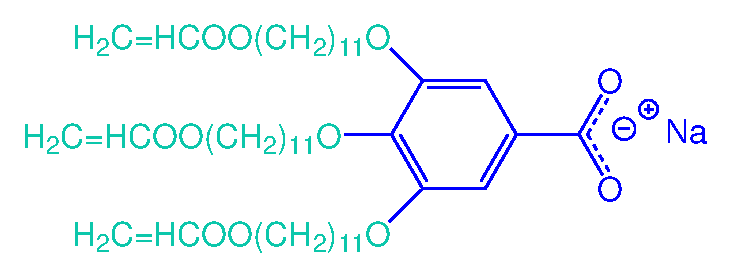
\includegraphics[width=\textwidth]{NaGA3C11_wedge.eps}
              \vspace{0.05cm}
              \caption{}~\label{fig:monomer}
      \end{subfigure}
%      \begin{subfigure}{.3\textwidth}
%              \centering
%              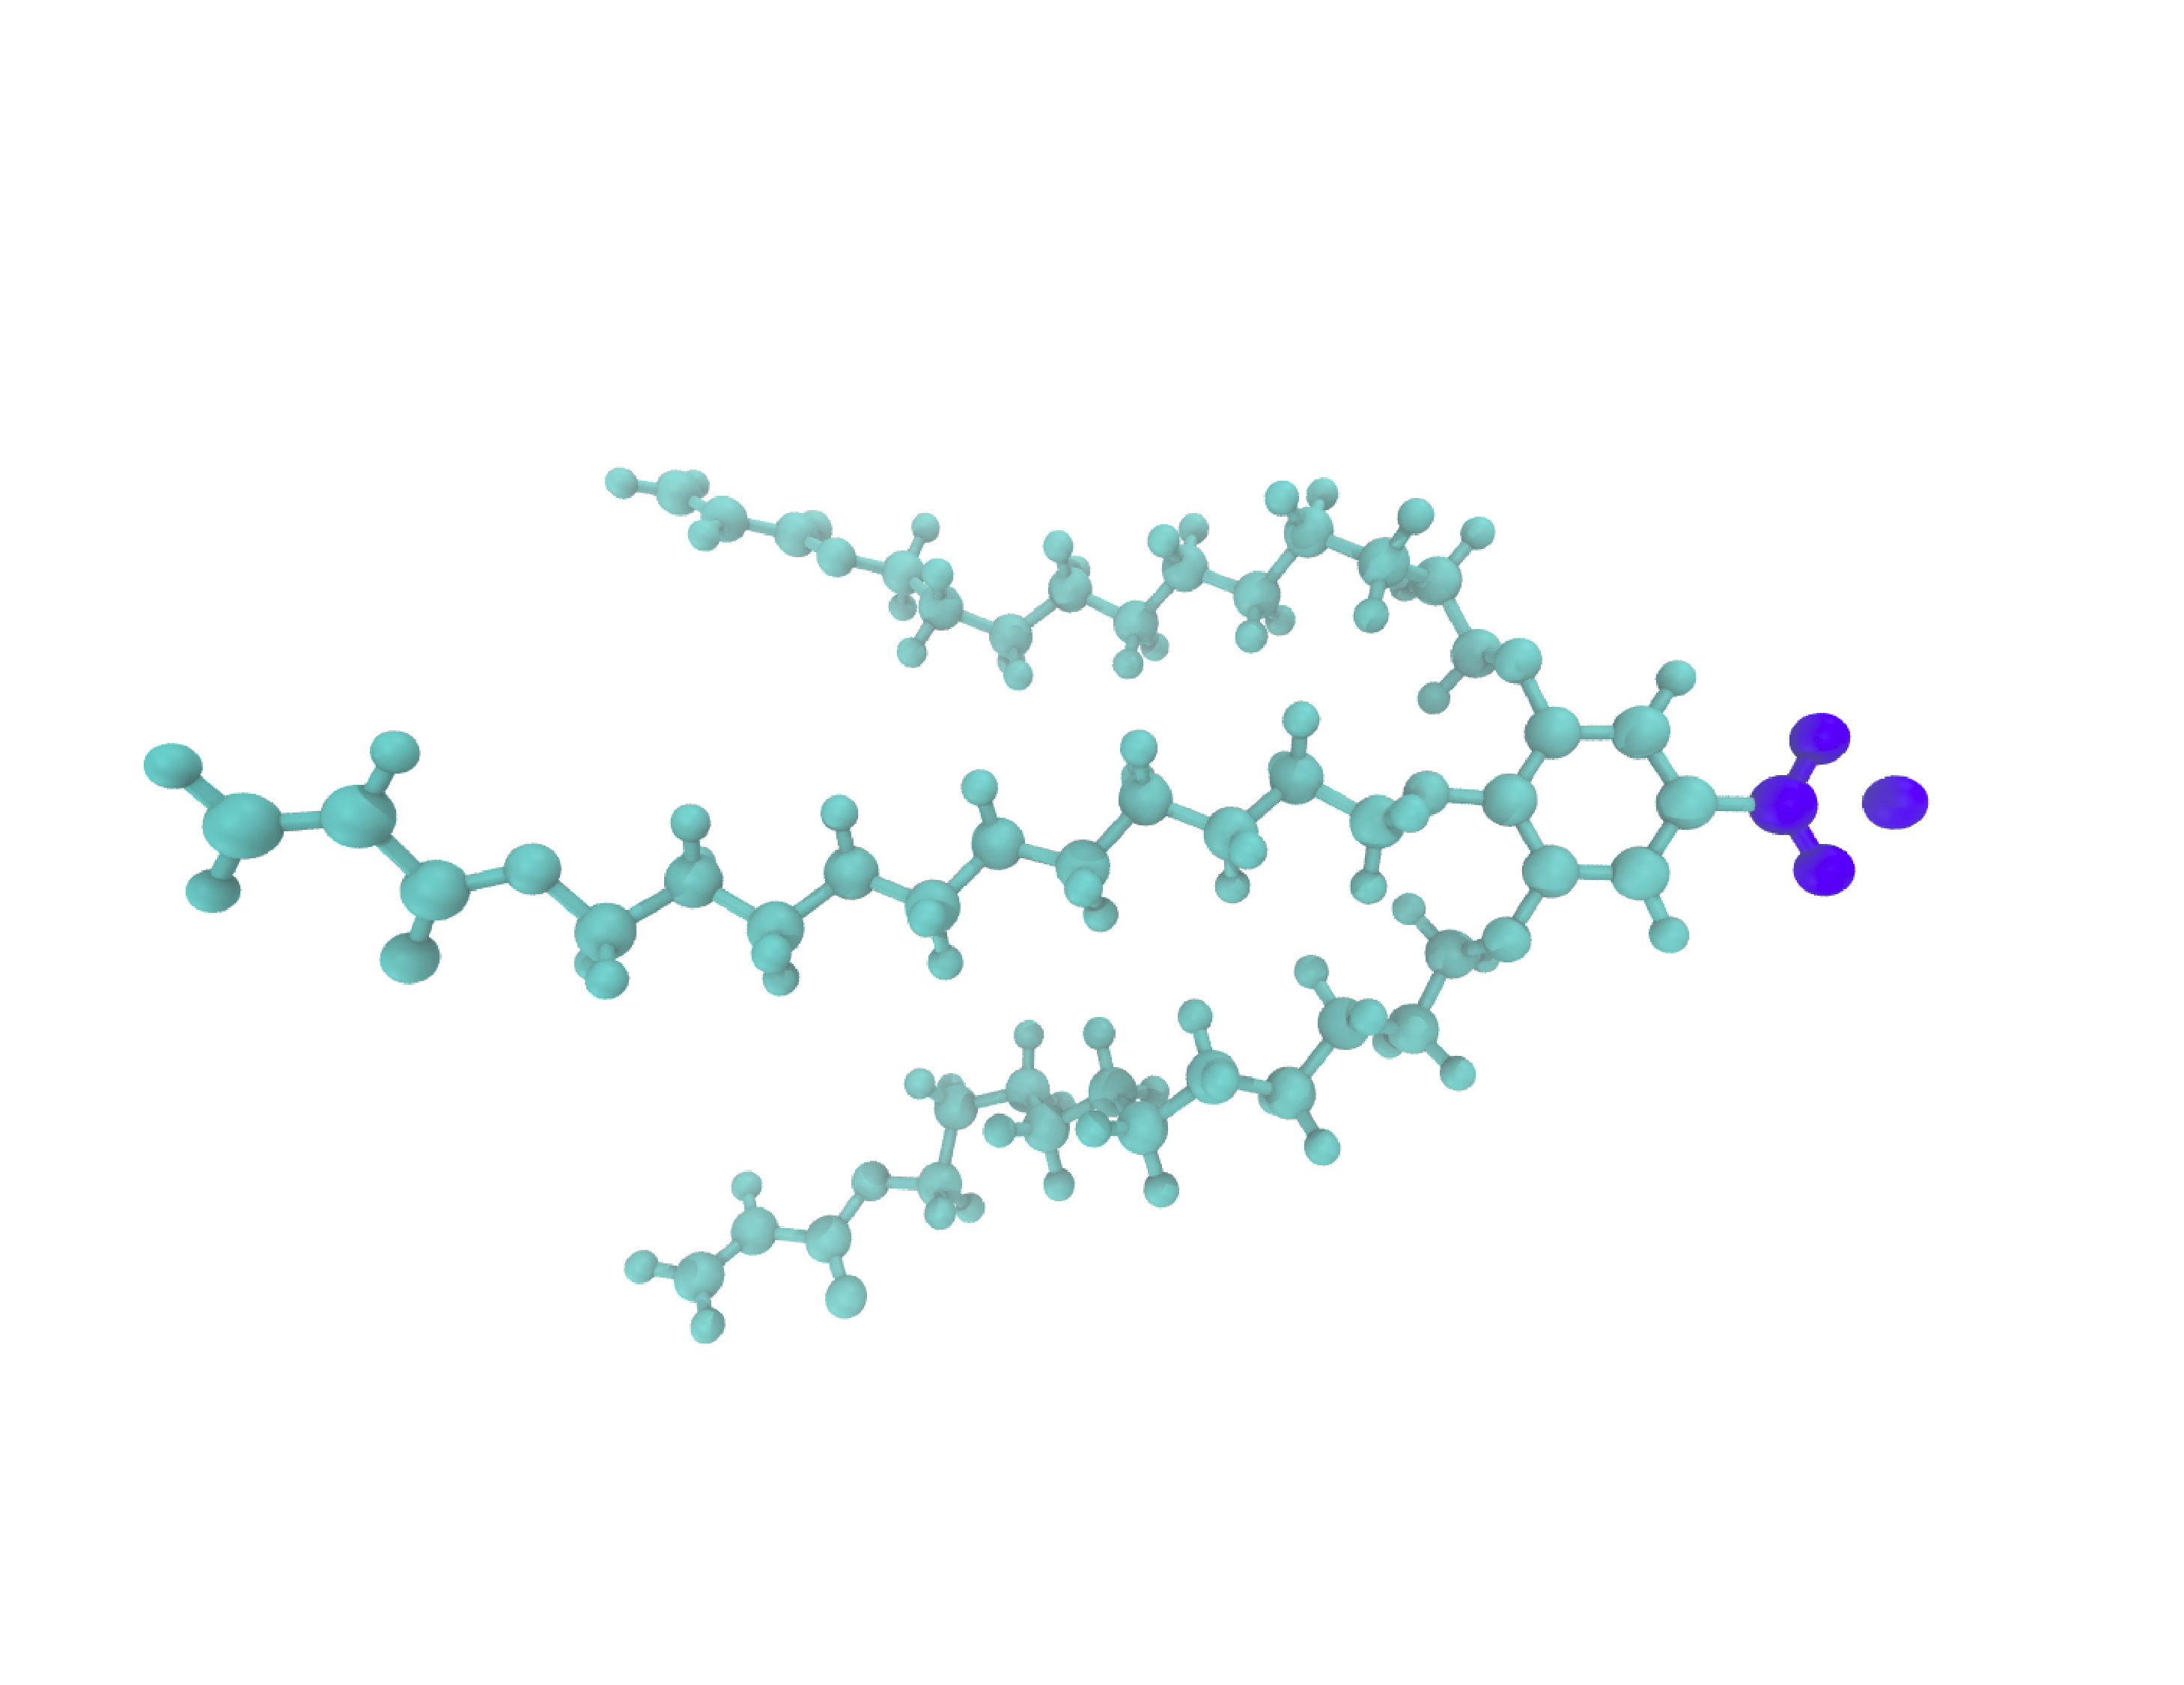
\includegraphics[width=\textwidth]{monomer_twocolor.pdf}
%              \caption{}~\label{fig:atomistic_monomer}
%      \end{subfigure}
%      \begin{subfigure}{0.3\linewidth}
%              \centering
%              
\includegraphics[width=0.6\textwidth]{wedge_thick.pdf}
%              \caption{}~\label{fig:wedge}
%      \end{subfigure}
              \begin{subfigure}{0.325\linewidth}
              \centering
              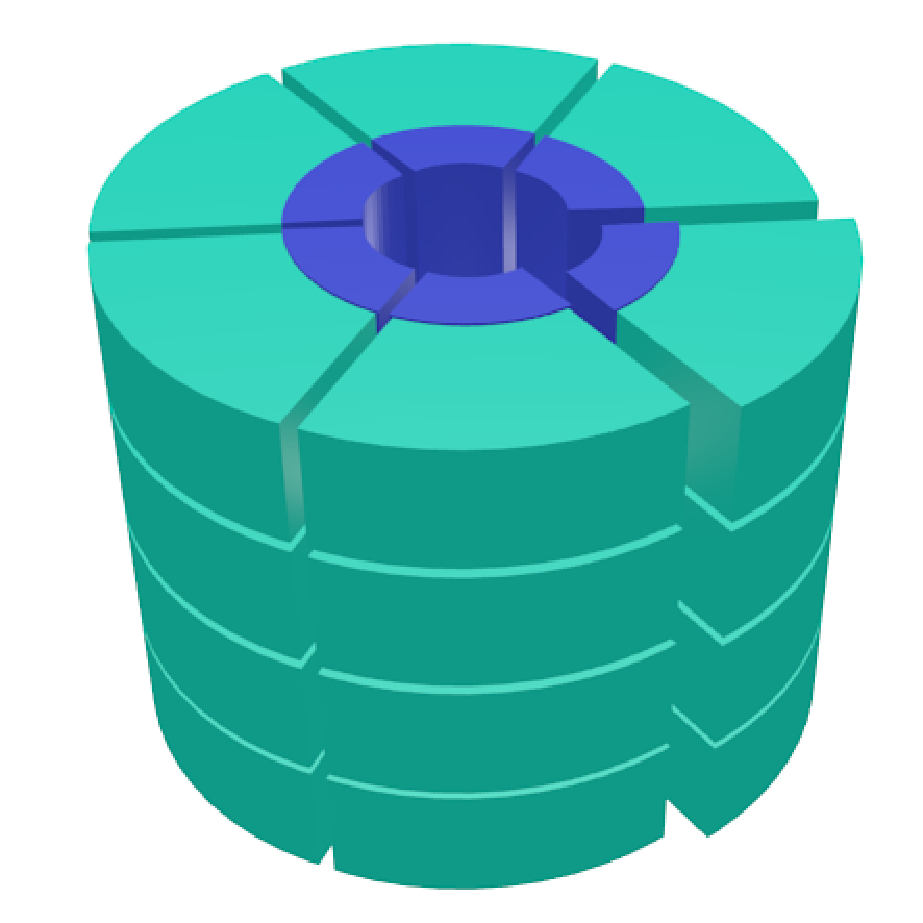
\includegraphics[width=0.6\textwidth]{columns.pdf}
              \caption{}~\label{fig:wedge_layer}
      \end{subfigure}
      \begin{subfigure}{0.325\linewidth}
              \centering
              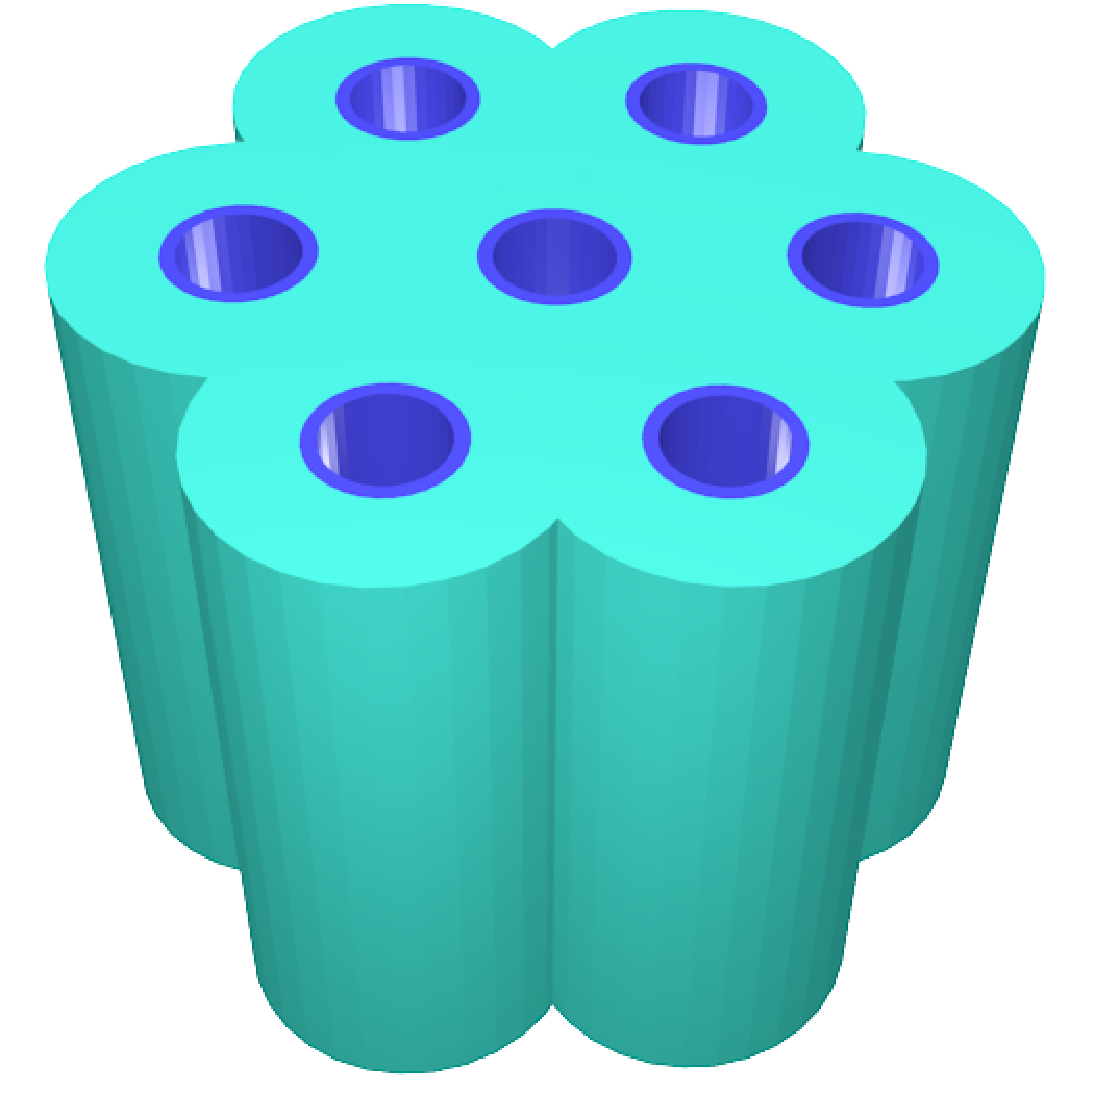
\includegraphics[width=0.6\textwidth]{hexagonal_packing.pdf}
              \caption{}~\label{fig:hex_packing_simple}
      \end{subfigure}
      \caption{(a) The LLC monomer Na-GA3C11 exhibits wedge-like character. (b) 
      Monomers stack on top of each other to create columns with short range order,
      then assemble into pores with hydrophilic head groups (blue) facing towards 
      the pore center. (c) The pores assemble into hexagonally packed columnar
      mesophases.}~\label{fig:assembly}
      \vspace{-0.5cm}
  \end{figure}
  
  I evaluated a number of different initial column architectures. I stacked 
  monomers in parallel displaced and sandwiched configurations, two possible
  $\pi$-$\pi$ stacking modes that might occur between monomer phenyl groups.
  ~\cite{sinnokrot_estimates_2002} I also varied the initial distance between
  stacked monomers, $d$. I chose $d$ values of 3.7~\AA, based on experimental
  WAXS measurements, as well as 5 \AA~as a test of its sensitivity.
  
  My model's geometry is most consistent with experiment for systems built
  with 5 columns per pore and monomers initially stacked 3.7 \AA~apart
  (see Figure~\ref{fig:p2p}). I equilibrated systems with 4, 5, 6, 7 and 
  8 columns per pore. The pore spacing of 5 column-per-pore systems agree
  well with experiment. 6 column-per-pore systems built with $d$ = 5 \AA~appear
  to yield an experimentally consistent pore spacing however, the equilibrated
  distance between stacked monomers stay close to 5 \AA~which is inconsistent
  with experiment. In general, the equilibrated distance between monomers stays
  close to its initial value. 
  
  \begin{wrapfigure}{L!}{0.5\textwidth}
    \centering
    \vspace{-0.5cm}
    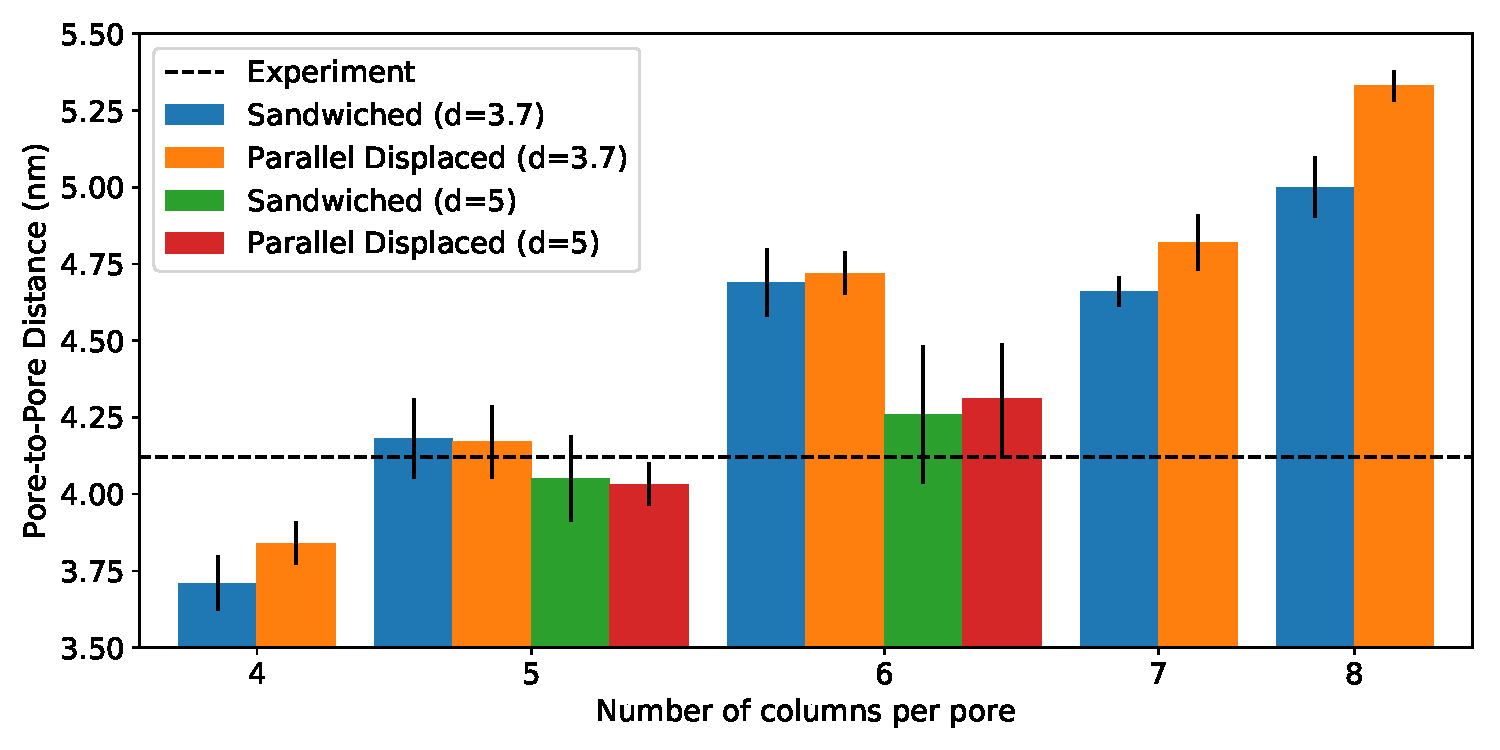
\includegraphics[width=\linewidth]{p2p.pdf}
    \caption{Systems with 5 columns per pore have equilibrated pore spacings
            closest to the experimental value of 4.12 nm. The equilibrated 
            pore spacing of the model increases as the number of columns in
            each pore increases.}~\label{fig:p2p}
    \vspace{-1.25cm}
  \end{wrapfigure}
  
%  \noindent On timescales that we can reasonably simulate, our equilibrated
%  structures show some initial configuration dependence. 
%  \begin{itemize}
%    \item All of the systems used to generate Figure~\ref{fig:p2p} are at 
%    least metastable.
%    \item We observe no large scale rearrangements that would be necessary
%    for all structures to converge to the same equilibrium structure. 
%  \end{itemize}

  I further validated the structure of our molecular model by verifying 
  its consistency with five major reflections present in the experimental
  WAXS pattern. Using MD trajectories, we simulated X-ray diffraction (XRD)
  patterns that we could compare to the WAXS data by taking the appropriate
  cross-section of the time-averaged 3D structure factor. The five major 
  reflections and the structural features leading to them are summarized
  and described in the caption of Figure~\ref{fig:WAXS_comparison}. Note that
  none of the models simulated to this point could reproduce R-double.   
  
  It is necessary to add a small amount of water to the model in order to 
  fully reproduce all features of the WAXS pattern (see Figure~\ref{fig:solvated_XRD}).
  I obtain the most experimentally consistent structure when I build systems
  in the parallel displaced configuration with 1 wt\% water added to the pores. 
  This is the only configuration that gives rise to the R-double feature without
  imposing some kind of position restraint. R-double appears because 
  vertically adjacent monomer head groups hydrogen bond with shared water molecules,
  causing them to be drawn closer together. When multiple pairing interactions
  occur in series along the same pore axis, the center of masses of the pairs 
  are spaced apart at twice the $\pi$-stacking distance. The necessity of water
  in my model suggests that the membrane synthesized by Feng et al.
  ~\cite{feng_scalable_2014,feng_thin_2016} was slightly hydrated due to water 
  molecules leached from surroundings by the hydroscopic monomers. Similar 
  suspicions have been voiced by experimentalists in unpublished communications.
  
  \begin{wrapfigure}{R!}{0.65\textwidth}
  	\centering
  	\vspace{-0.5cm}
    \begin{subfigure}{0.49\linewidth}
    	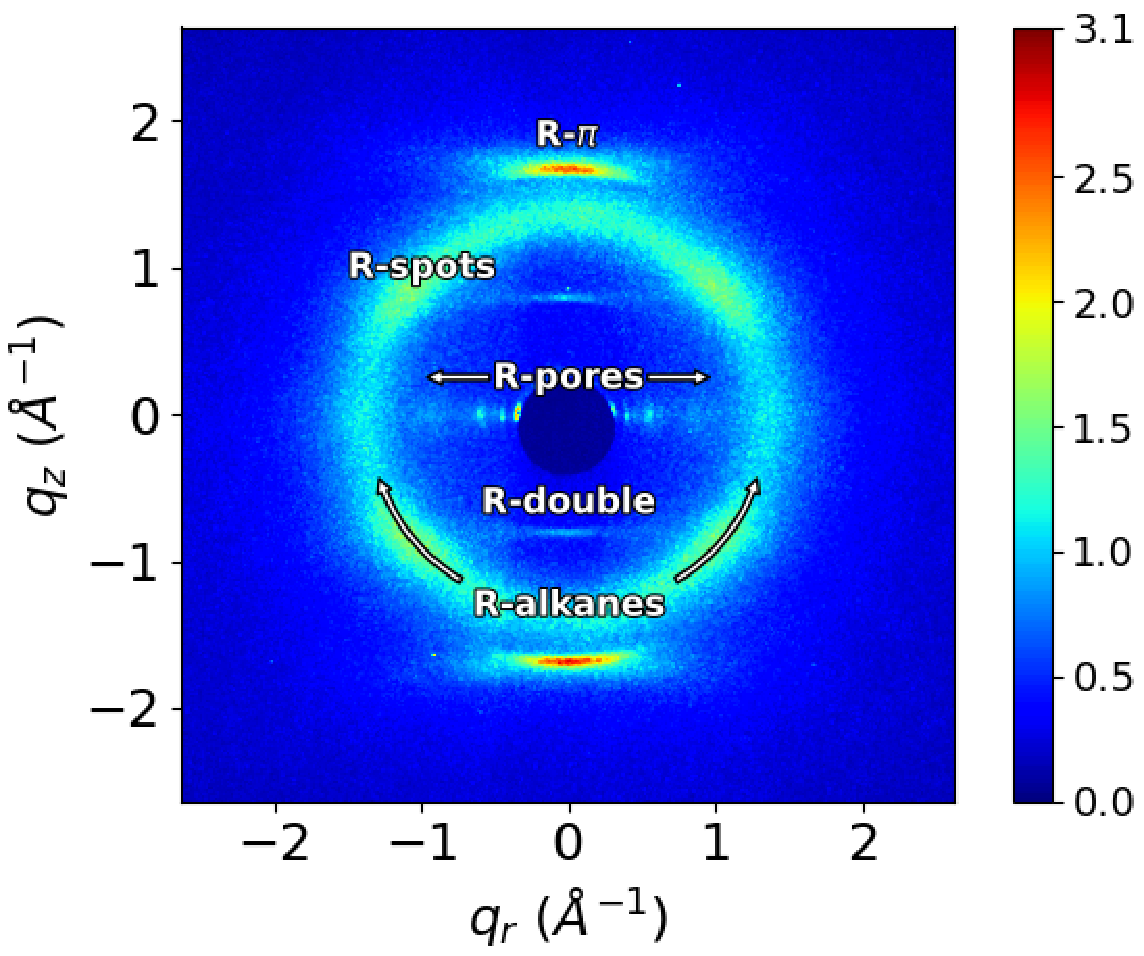
\includegraphics[width=\linewidth]{WAXS_annotated_words.pdf}
        \caption{Experiment}\label{fig:WAXS}
    \end{subfigure}
	\begin{subfigure}{0.49\linewidth}
        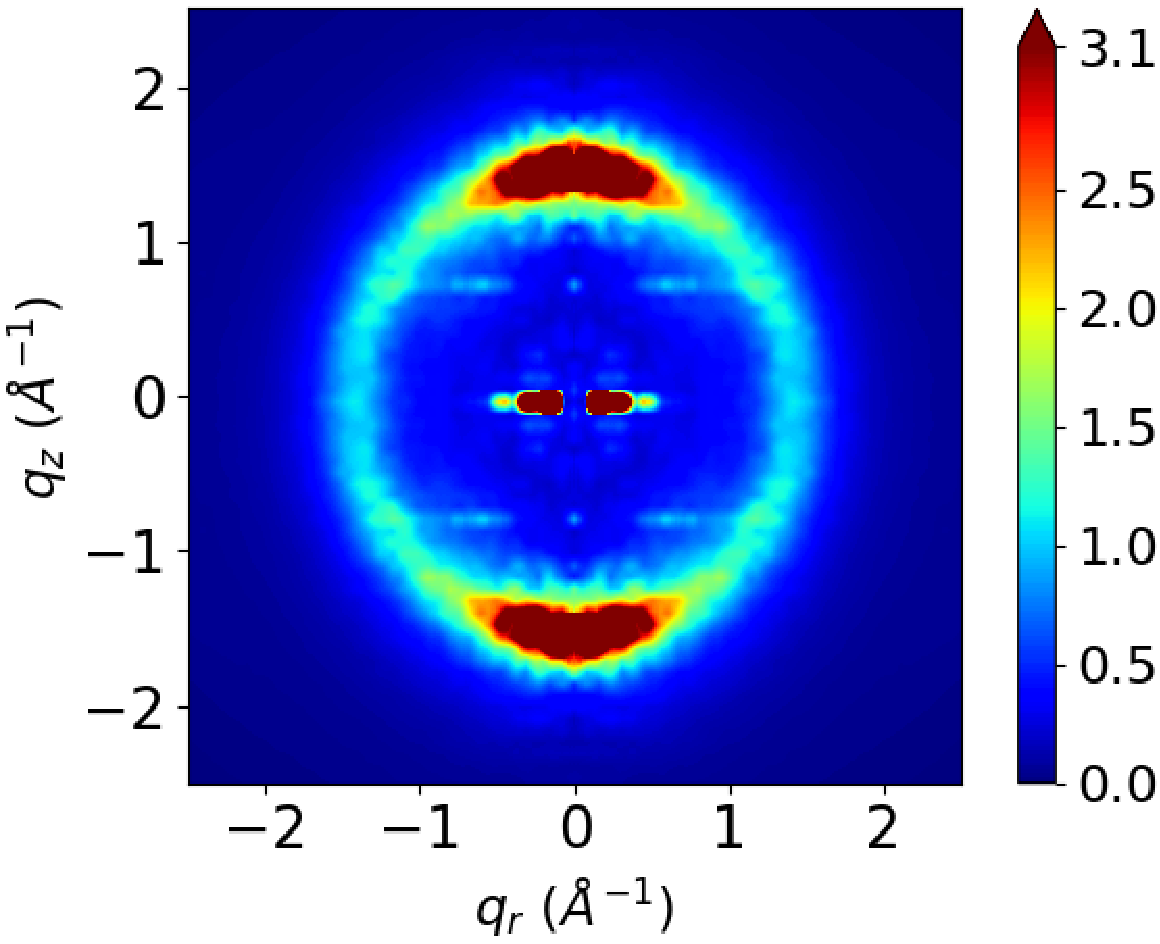
\includegraphics[width=\linewidth]{solvated_offset_rzplot_1.pdf}
        \caption{Simulation}\label{fig:solvated_XRD}   
	\end{subfigure}
    \caption{(a) 2D-WAXS gives details about repeating features on the order of
    angstroms. Explanations for each of the 5 major reflections present are
    as follows: (R-$\pi$) Aromatic head groups $\pi-\pi$ stack 3.7 \AA~apart. 
    (R-double) Monomer head groups associate into pairs by hydrogen bonding with
    a shared water molecule. R-double does not appear in dry systems. 
    (R-alkanes) Alkane chain tails pack 4.5 \AA~apart. (R-spots) Monomer tails
    pack hexagonally. (R-pores) The pores are spaced 4.12 nm apart and pack 
    hexagonally. (b) We obtain a maximally consistent match between simulated
    XRD patterns and experimental WAXS data when we build systems in the 
    parallel displaced configuration with 1 wt \% water included in the pores.
    }\label{fig:WAXS_comparison}
    \vspace{-0.75cm}
 \end{wrapfigure}
 
  On the timescales that one can reasonably simulate, my model exhibits slow 
  dynamics. Consequently, there are very few uncorrelated frames in the 
  trajectories which leads to noise and sharpened reflections in the simulated
  XRD patterns. One can overcome this issue by combining the structure factors
  generated from an ensemble of simulated trajectories each produced
  from an ensemble of uncorrelated initial configurations. One can create 
  decorrelated initial configurations by randomly displacing monomer columns in
  the $z$-direction.
 
  Perhaps the most important conclusion from my structural work is that the 
  chemical composition of the pores is relatively insensitive to the initial 
  configuration. In Figure~\ref{fig:overlaid_densities}, I plot the radial 
  distribution function of various monomer components as a function of distance
  from the closest pore center. All are qualitatively similar meaning that a 
  solute placed in any of these systems should experience a similar chemical 
  environment. Although we will move forward with our most promising 
  configuration, this is an important finding since it implies that one does
  not need to apply the same level of rigor when screening new monomers.
  
  \begin{figure}[!htb]
  \centering
  \begin{subfigure}{\textwidth}
  %BJC: probably change this legend to `d = x Angstroms` instead of 
  % disordered/ordered, since I don't have space to talk about ordered / disorderd configurations (requires 
  % nematic order parameter to give a complete justification of the names)
  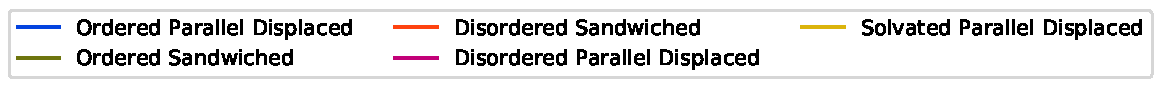
\includegraphics[width=\textwidth]{regional_density_legend.pdf}
  \end{subfigure}
  \begin{subfigure}{0.32\textwidth}
        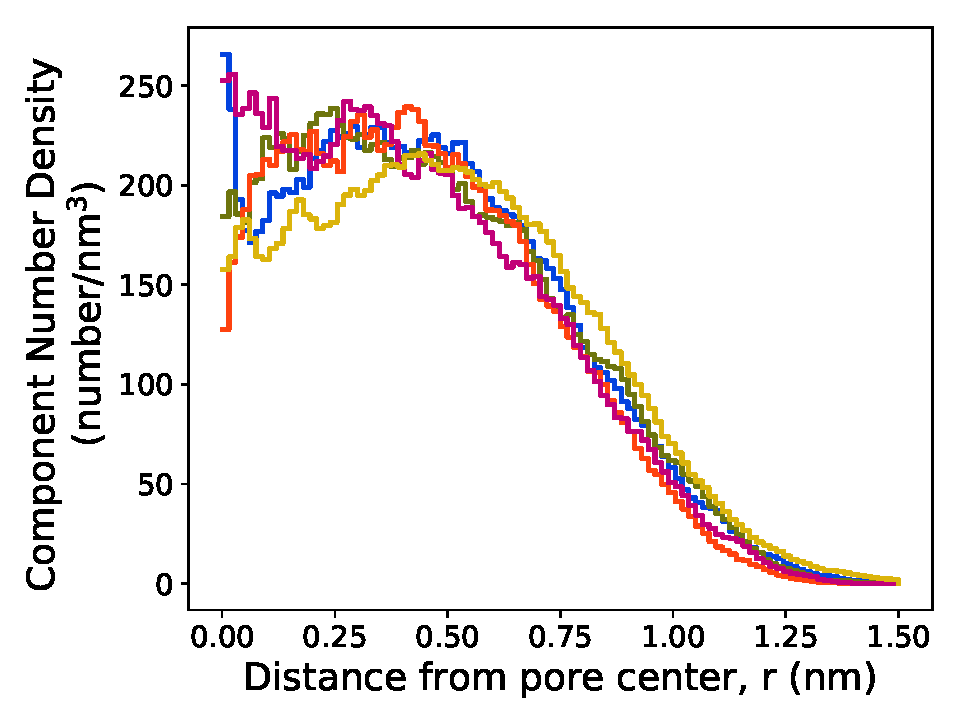
\includegraphics[width=1\linewidth]{head_group_density.pdf}
        \caption{Head Groups}
        \label{fig:head_groups_regional_density}
  \end{subfigure}
  \begin{subfigure}{0.32\textwidth}
        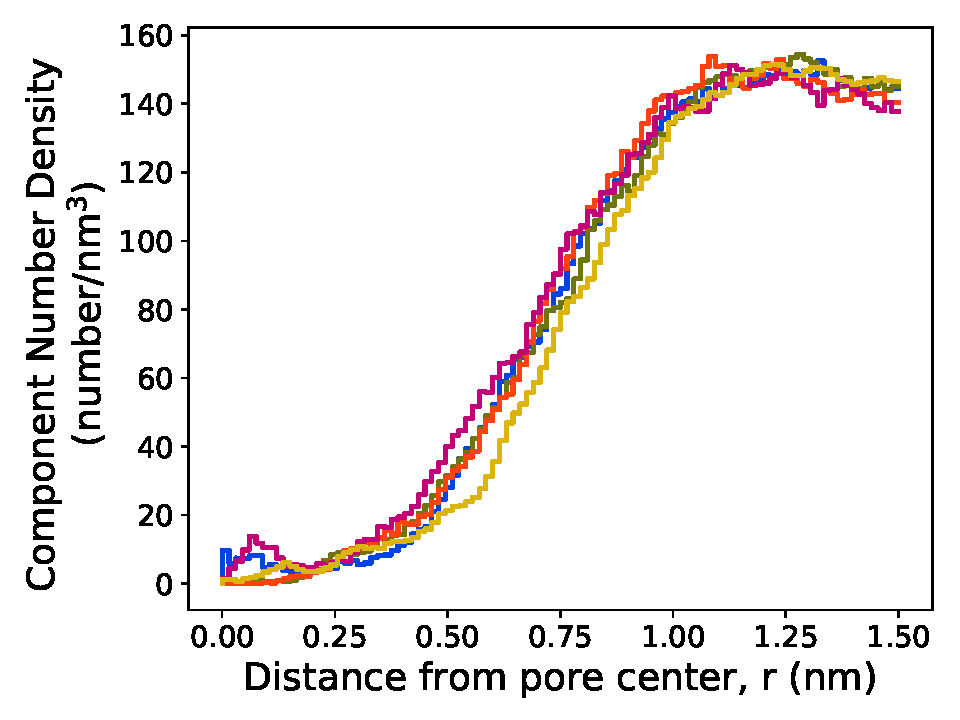
\includegraphics[width=1\linewidth]{tails_density.pdf}
        \caption{Tails}
        \label{fig:tails_regional_density}
  \end{subfigure}
  \begin{subfigure}{0.32\textwidth}
        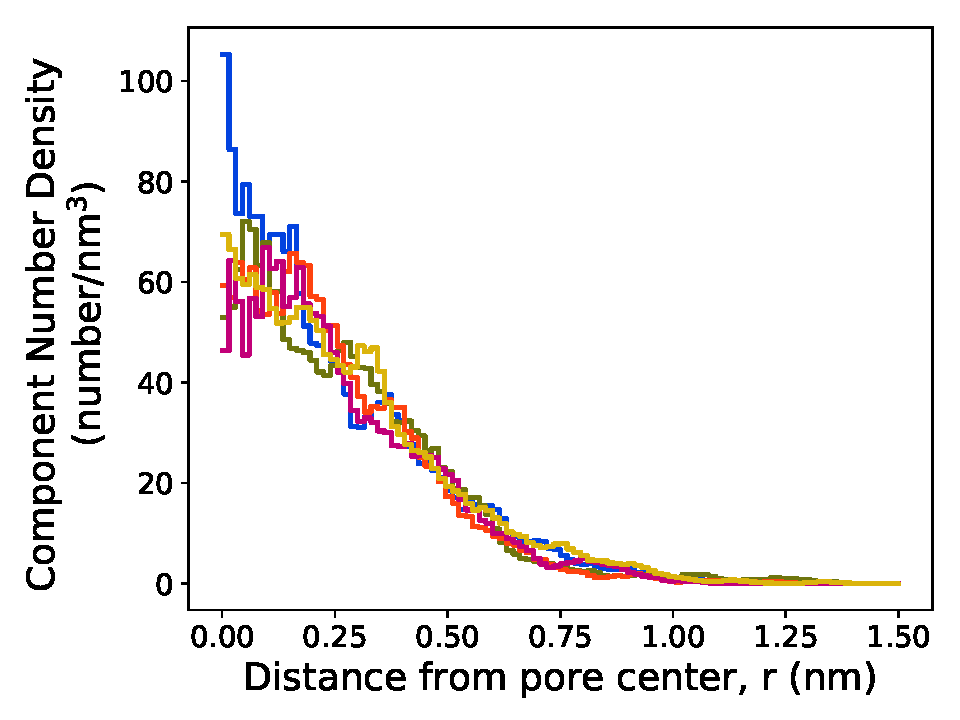
\includegraphics[width=1\linewidth]{sodium_density.pdf}
        \caption{Sodium Ions}
        \label{fig:sodium_regional_density}
  \end{subfigure}
  %MRS2: important consquence of all radian distribution functions being similar is that we should get useful transport details even if we didn't get the structure exactly right. 
  \caption{In all systems studied, the component radial distribution functions are similar.
      They exhibit a composition gradient transitioning from the hydrophilic to the hydrophobic
          regions. The biggest differences are at r=0 where noise is higher due to
          decreased sampling. The center of the pore is not hollow, but contains sodium ions and
          head groups, even when the system is solvated. This architecture may impede transport in
          the real system in a chemically-dependent manner.
          The solvated system has a lower density of head groups near the
          pore center which is likely due to the swelling that is necessary in order to fit water
          molecules in the pore region.}~\label{fig:overlaid_densities}
  \vspace{-0.5cm}
  \end{figure}
  
  \noindent \textbf{\large Objective 2:} \textit{\large Determine transport mechanisms} (\textcolor{green!40!olive}{\textbf{Complete}})
  
  \noindent A manuscript based on the work presented towards this objective is under 
  review for publication in the Journal of Physical Chemistry B.

  I added additional water to the most experimentally consistent structural
  model in order to create a higher water content H\textsubscript{II} phase
  model. Researchers have synthesized the H\textsubscript{II} phase using 
  the NaGA3C11 monomer with water contents ranging from 7 - 20 wt\%, with 
  close to 10 wt\% being the most common.~\cite{smith_ordered_1997,zhou_supported_2005} 
  However, Resel et al. stated that the system is likely fully hydrated at
  7 wt \% water with additional water trapped in defects between hexagonal
  mesophases.~\cite{resel_structural_2000} Consequently, we chose to build
  two systems with 5 and 10 wt\% water.
  
  Upon simulating each system, we observed that water partitions into the
  distal tail region. Based on the radial distance from the pore center where 
  the minimum water density occurs, we defined the distal tail region to 
  be greater than 1.5 nm from any pore center. There is approximately a 3:2
  ratio of water in the pores to water in the distal tails. Due to the wedge
  shape of the monomers, the distal tail region has a relatively low density
  leaving space for water molecules to fill.
  
  \begin{wrapfigure}{l}{0.65\textwidth}
  \centering
%  \vspace{-0.3cm}
%  \begin{subfigure}{0.325\textwidth}
%  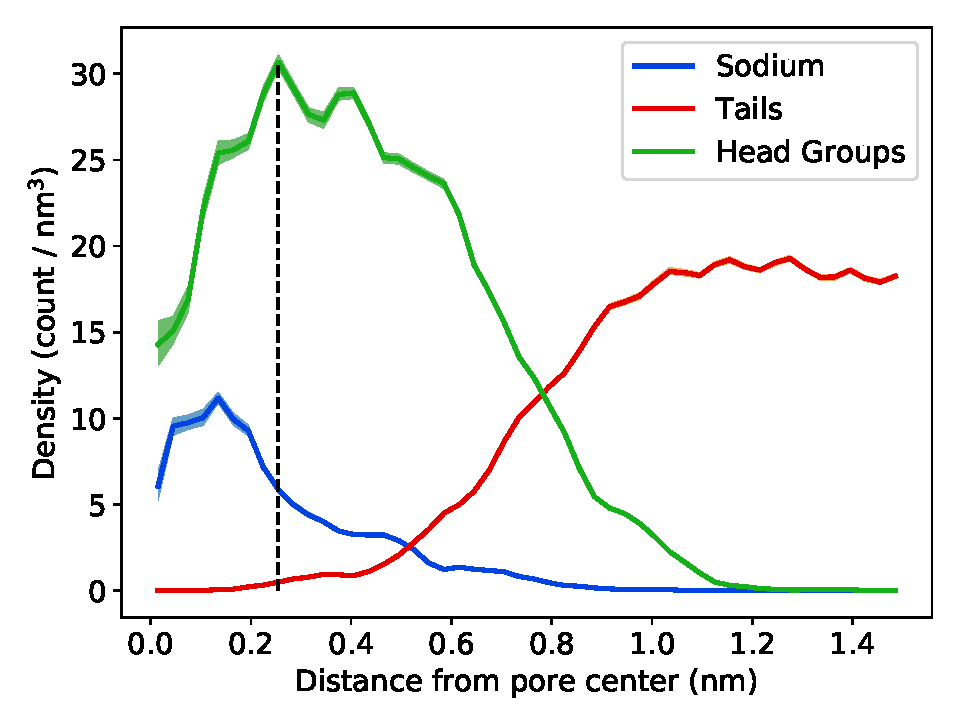
\includegraphics[width=\textwidth]{component_density_dry.pdf}
%  %BJC: simulation is extended to smooth out these curves
%  \caption{Dry System}\label{fig:component_density_dry}
%  \end{subfigure}
%  \begin{subfigure}{0.45\textwidth}
%  \vspace{-0.5cm}
%  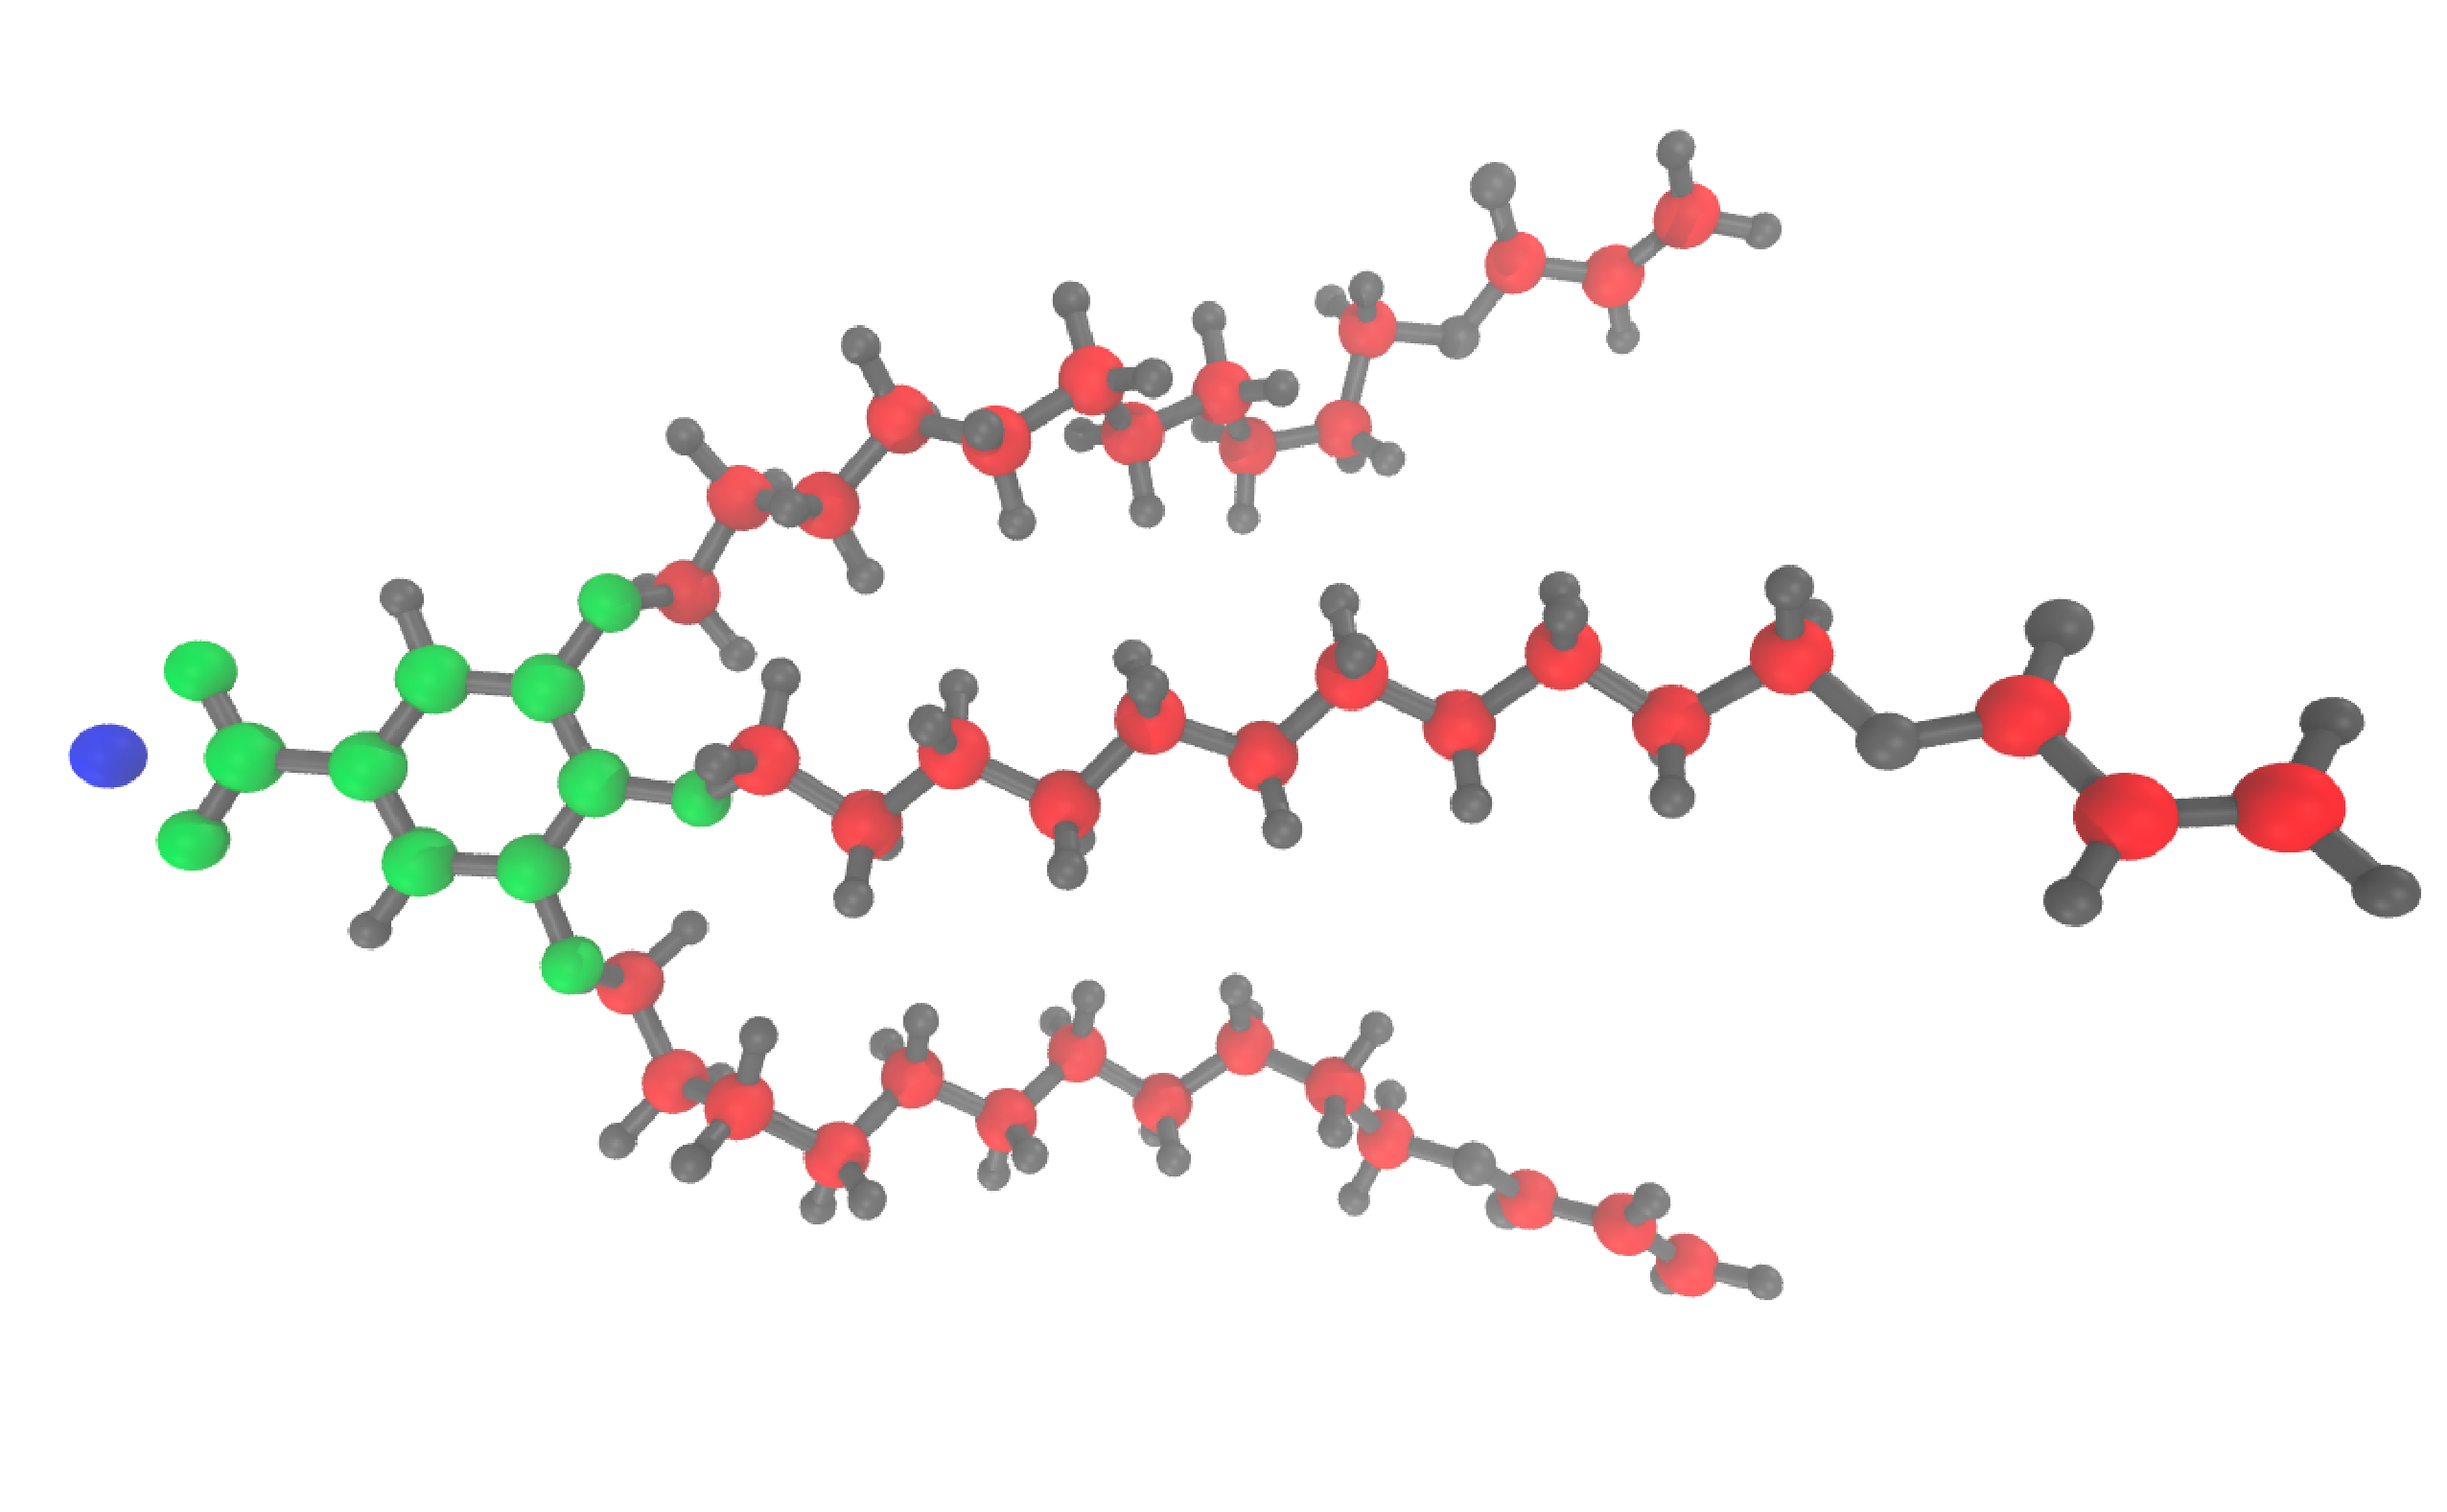
\includegraphics[width=\textwidth]{monomer_color_coded.pdf}
%  \label{fig:monomer_color_coded}
%  \end{subfigure}
  \begin{subfigure}{0.49\linewidth}
  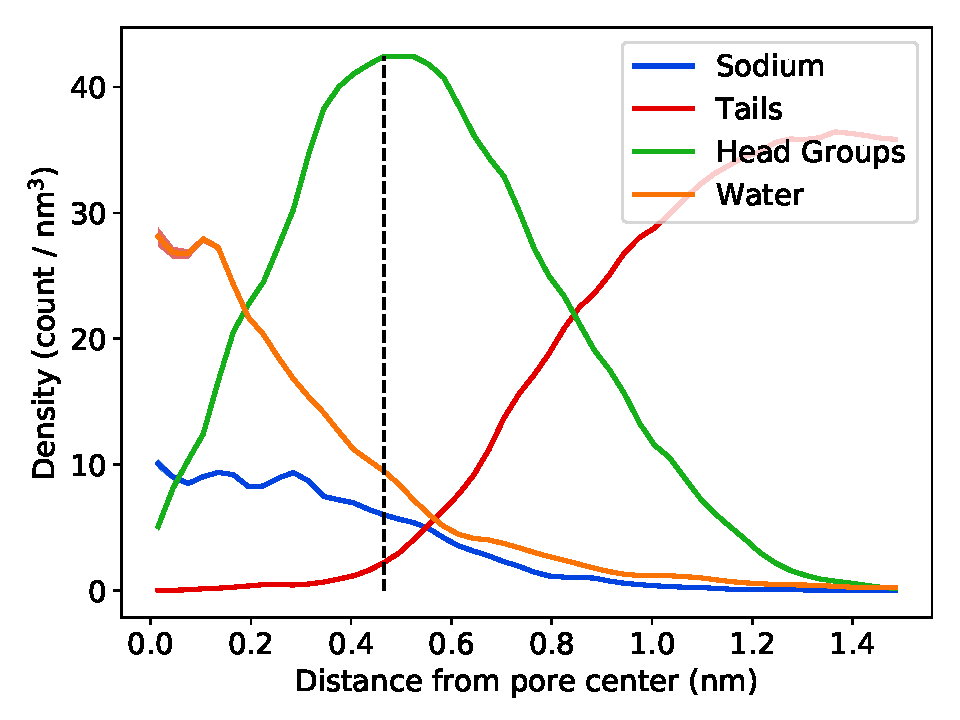
\includegraphics[width=\linewidth]{component_density_5wt.pdf}
  \caption{5 wt\% water}\label{fig:component_density_5wt}
  \end{subfigure}
  \begin{subfigure}{0.49\linewidth}
  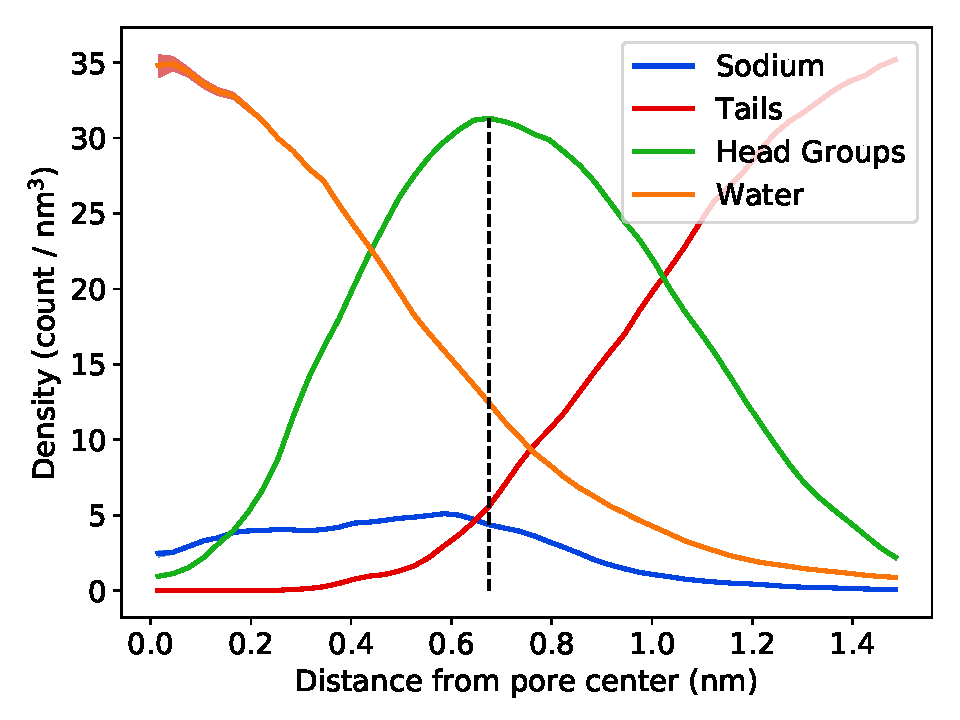
\includegraphics[width=\linewidth]{component_density_10wt.pdf}
  \caption{10 wt\% water}\label{fig:component_density_10wt}
  \end{subfigure}
  \caption{The radial densities of various monomer components paint a
  picture of the pore topology where the pore centers are primarily 
  composed of water, sodium ions and head groups to varying degrees
  depending on total water composition.
  %MRS2: there's actually a lot of head groups in the pores except at the very center.  Does the sentence above
  %MRS2: communicate that well? 
  %BJC2: rephrased.
  The monomer groups labeled in each plot correspond to
  the color-coded monomer pictured in Figure~\ref{fig:HII_mon}. All RDFs
  represent the number of atoms located at a given distance from the pore center
  normalized by the volume of the annular bin to which they belong. The black
  dashed lines are positioned so that they intersect with the maximum head group
  density. (a) In the 5 wt \% system, monomer head groups are situated about 0.45 nm
  from the pore center. Sodium and water are densest near the pore center 
  (b) Monomers in the 10 wt \% system retreat an additional 0.2 nm to make room
  for more water. Water is densest at the pore center, but sodium ion density
  peaks closer to the head groups since many stay bound to carboxylate groups.}\label{fig:component_densities}
  \vspace{-0.5cm}
  \end{wrapfigure}
  
  The pores of the H\textsubscript{II} phase are a mixture of water, sodium
  ions and monomer head groups. Water is densest at the pore center ($r = 0$).
  The maximum density of head groups occurs 0.45 and 0.65 nm from the pore 
  center in the 5 and 10 wt\% water systems respectively (see 
  Figure~\ref{fig:component_densities}).
  
  %There are almost no head groups 
  %occupying the pore center.
  %MRS2: I guess that's not entirely clear to me. Yes, at R=0, but most of the pore volume is at R=0.2-0.4, and there are a lot of head groups there.  There might be a general issue of confusion between ``pore center'' and ``pore regions''
  %BJC2: Avoiding the confusion. I think saying this makes more sense when comparing
  %directly to the dry system which has a significant head group density at R=0.
    
  Water and sodium transport is significantly faster in the less crowded 
  10 wt\% water pores. The mean squared displacement (MSD) of water is about
  51 times higher and the MSD of sodium is about 49 times higher compared to
  the 5 wt\% system. In general we observe similar solute transport mechanisms
  in the 5 and 10 wt\% water systems but on different time scales.
    %BJC: might as well leave 5 wt% data in there.
%    \item Therefore, we focus the remainder of this discussion on the 10 wt\%
%    water system since we were able to collect a larger quantity of mechanistic
%    data from the solute trajectories.
  
  %MRS2: not great thesis statement.  Thesis statements should be trying to convince reader - this is just listing something you did. 
  %BJC2: tried again.
  I explored the influence of a solute's chemical functionality on its 
  transport properties within the H\textsubscript{II} nanopores using simulations
  of 20 different small polar solutes (see Table~\ref{fig:solute_table}).
  For each solute, I created a separate initial configuration and placed 6 
  solutes, equally spaced in $z$, in each nanopore. This gave a sufficient
  number of solute trajectories from which to generate statistics while 
  maintaining a low degree of interaction between solutes. 
  
  % Unnecessary details
  % After a 5 ns equilibration, we allowed the solutes to simulate for
  % 1 microsecond. 
  
  \begin{figure}
  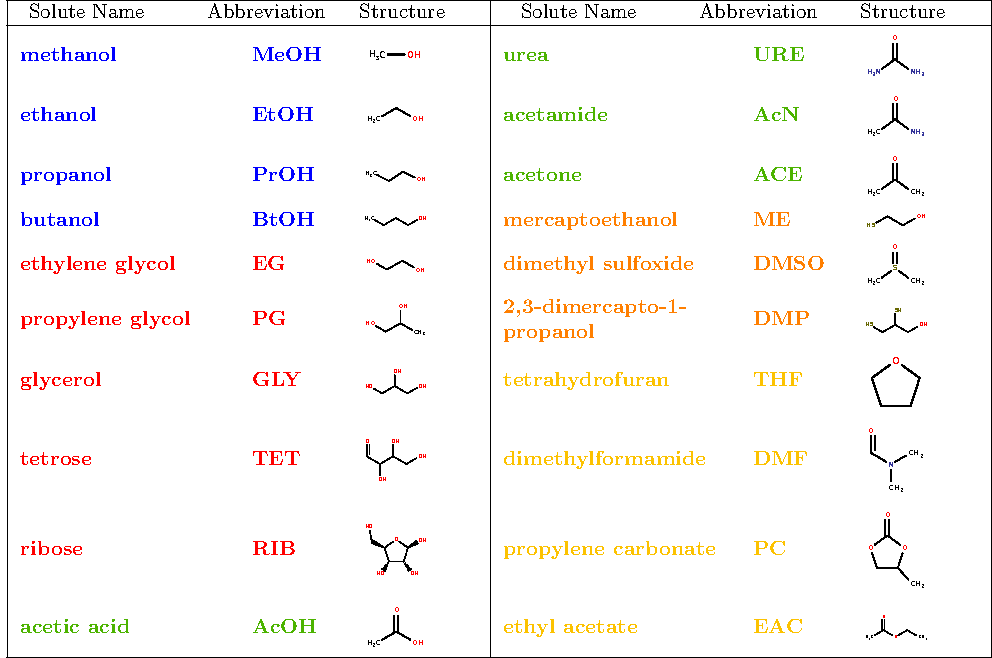
\includegraphics[width=\textwidth]{solute_table.pdf}
  \caption{The solutes studied in this work along with the abbreviations used
  in subsequent figures and their chemical structures. Solutes are color-coded
  according to similarities in their structure. Blue corresponds to simple 
  alcohols, red to diols, triols and sugars, green to ketone-like solutes, 
  orange to sulfur-containing solutes and yellow to solutes that can only accept
  hydrogen bonds but not donate.}\label{fig:solute_table}
  \vspace{-0.5cm}
  \end{figure}

%  \begin{wrapfigure}{R}{0.6\textwidth}
%  \centering
%  \begin{subfigure}{0.45\linewidth}
%  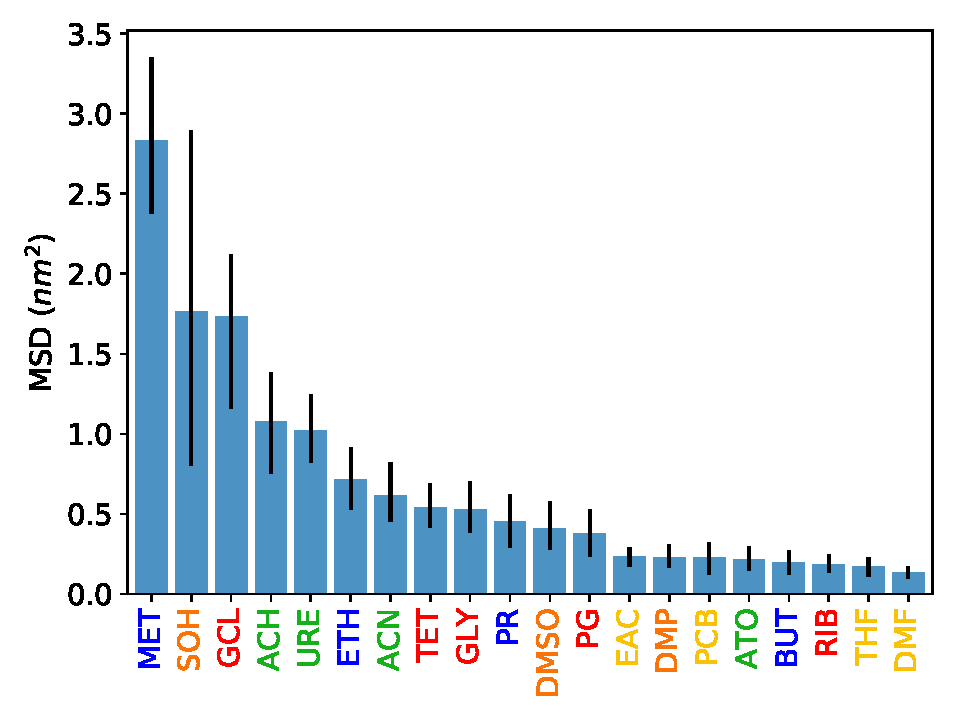
\includegraphics[width=\linewidth]{all_10wt_tamsds.pdf}
%  \caption{10 wt \% water}\label{fig:all_msds_10wt}
%  \end{subfigure}
%  \begin{subfigure}{0.45\linewidth}
%  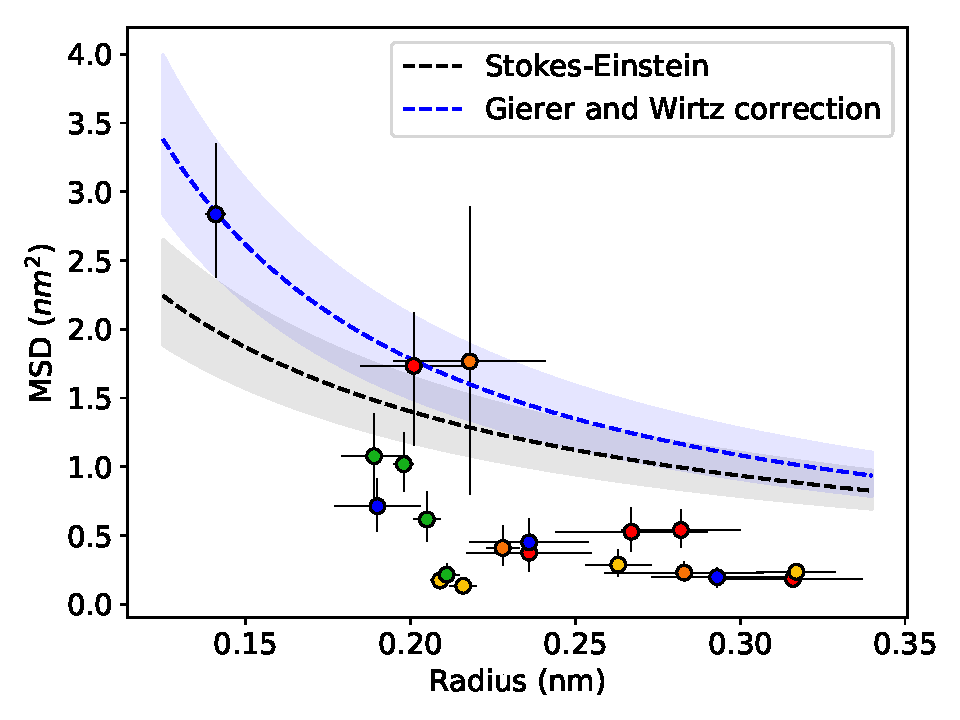
\includegraphics[width=\linewidth]{msd_radius_10wt.pdf}
%  \caption{10 wt \% water}\label{fig:msd_radius_10wt}
%  \end{subfigure}
%  \caption{The MSDs of solutes in the 5 wt \% water system (a) are significantly
%  smaller than those of the solutes in the 10 wt \% water system (b). The
%  MSDs are not a monotonic function of molecular size (c and d). A significant
%  number of solute MSDs fall below the theoretical lines predicted by the
%  Stokes-Einstein equation and Gierer and Wirtz' corrected Stokes-Einstein equation.
%  }\label{fig:msds}
%  \vspace{-1.5cm}
%  \end{wrapfigure}
    % 5 and 10 wt %
  
  The solute MSDs are not a monotonic function of solute size. In 
  Figures~\ref{fig:all_msds_5wt} and~\ref{fig:all_msds_10wt}, we plot
  the average MSD of each solute. In Figure~\ref{fig:msd_radius_5wt} 
  and~\ref{fig:msd_radius_10wt}, I plotted the solute MSDs against their
  molecular radius. Also plotted are theoretical curves which illustrate the 
  expected MSD of each solute if they were to travel unhindered. The 
  Stokes-Einstein equation with the correction factor of Gierer and 
  Wirtz~\cite{gierer_molekulare_1953} passes through methanol's MSD and
  radius in order to give an approximate frame of reference. The correction 
  factor attempts to include the effects of microfriction that begin to 
  play a role when solute size becomes on the order of solvent size. 
  Since methanol is small, I assume that it travels unhindered relative 
  to all other solutes. The theoretical line serves as an approximate 
  boundary between subdiffusive, Brownian and superdiffusive behavior.
  In the majority of cases, solute MSDs fall well below the theoretical
  lines and therefore are subject to more hindrance than methanol due to
  factors other than size.

  \begin{wrapfigure}{r}{0.65\textwidth}
  \centering
  \vspace{-0.4cm}
  \begin{subfigure}{0.45\linewidth}
  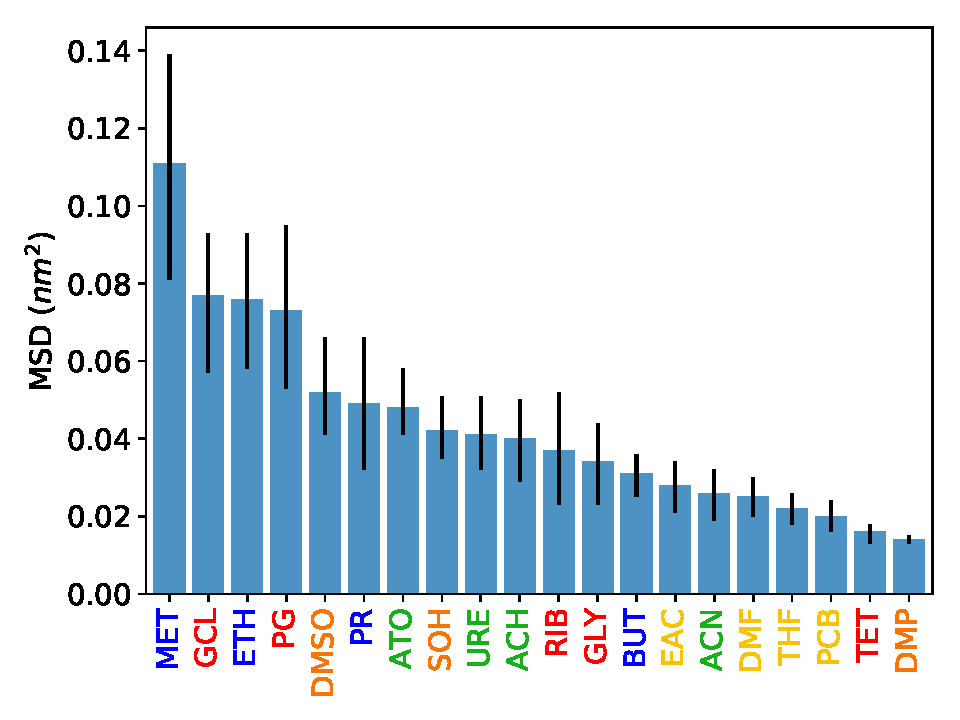
\includegraphics[width=\linewidth]{all_5wt_tamsds.pdf}
  \caption{5 wt \% water}\label{fig:all_msds_5wt}
  \end{subfigure}
  \begin{subfigure}{0.45\linewidth}
  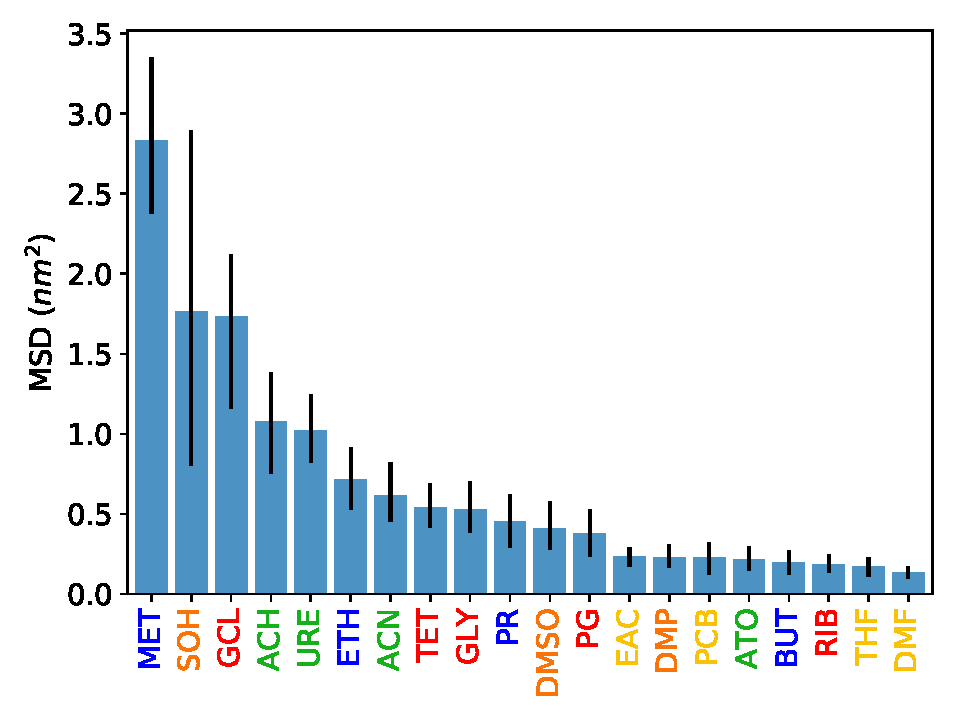
\includegraphics[width=\linewidth]{all_10wt_tamsds.pdf}
  \caption{10 wt \% water}\label{fig:all_msds_10wt}
  \end{subfigure}
  \begin{subfigure}{0.45\linewidth}
  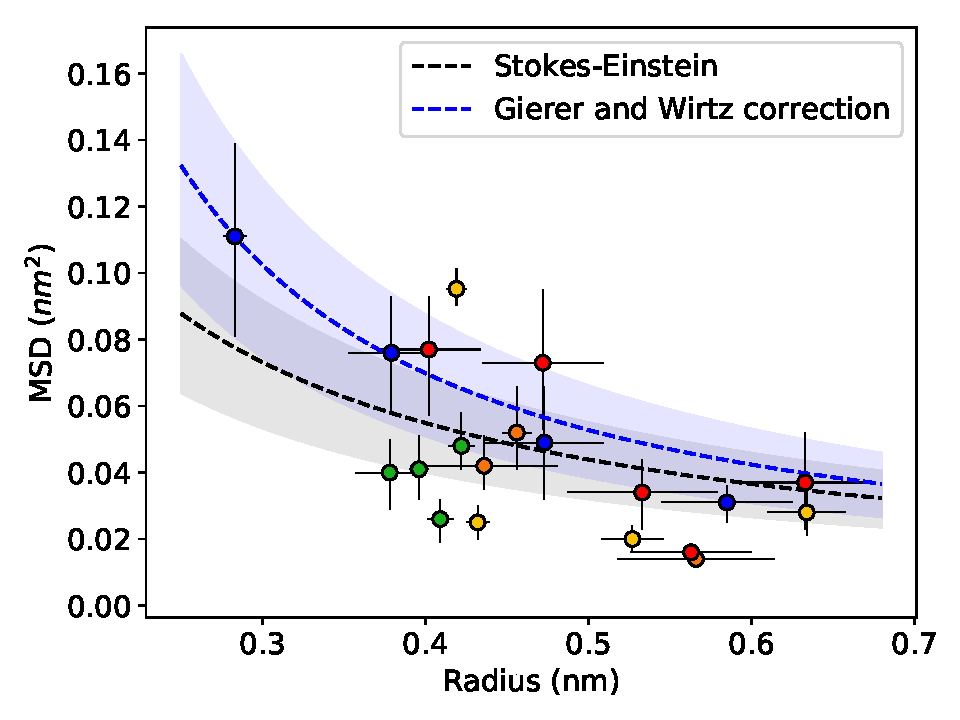
\includegraphics[width=\linewidth]{msd_radius_5wt.pdf}
  \caption{5 wt \% water}\label{fig:msd_radius_5wt}
  \end{subfigure}
  \begin{subfigure}{0.45\linewidth}
  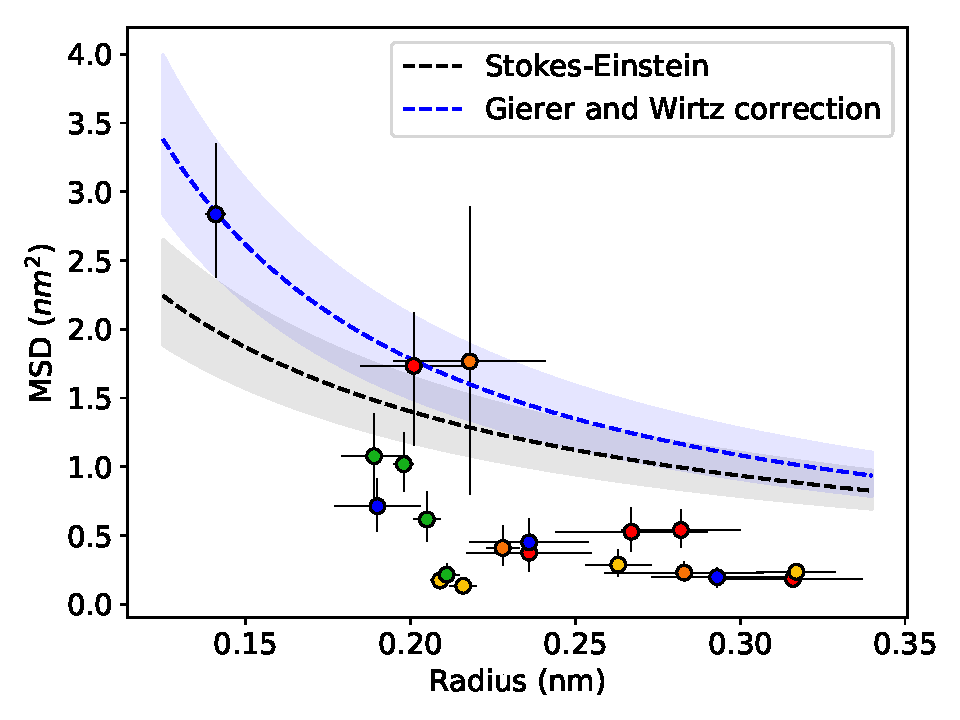
\includegraphics[width=\linewidth]{msd_radius_10wt.pdf}
  \caption{10 wt \% water}\label{fig:msd_radius_10wt}
  \end{subfigure}
  \caption{The MSDs of solutes in the 5 wt \% water system (a) are significantly
  smaller than those of the solutes in the 10 wt \% water system (b). The
  MSDs are not a monotonic function of molecular size (c and d). A significant
  number of solute MSDs fall below the theoretical lines predicted by the
  Stokes-Einstein equation and Gierer and Wirtz' corrected Stokes-Einstein equation.
  }\label{fig:msds}
  \vspace{-0.4cm}
  \end{wrapfigure}

  Intermittent hops between long periods of entrapment lead to subdiffusive
  solute transport behavior. As implied by Figures~\ref{fig:msd_radius_10wt} and~\ref{fig:msd_radius_5wt}, 
  most solutes move significantly slower than expected. In 
  Figure~\ref{fig:example_ztraces}, I've plotted the $z$-direction trajectory
  of three ethanol molecules. Typically, long periods of entrapment occur
  when ethanol molecules are far from the pore center, while there is a much 
  greater degree of mobility close to the pore center. The MSD curve averaged
  over all ethanol trajectories is shown in Figure~\ref{fig:example_msd}.
  The curve is sub-linear and thus subdiffusive.
  
  \begin{wrapfigure}{l}{0.6\textwidth}
  \centering
  \begin{subfigure}{0.49\linewidth}
  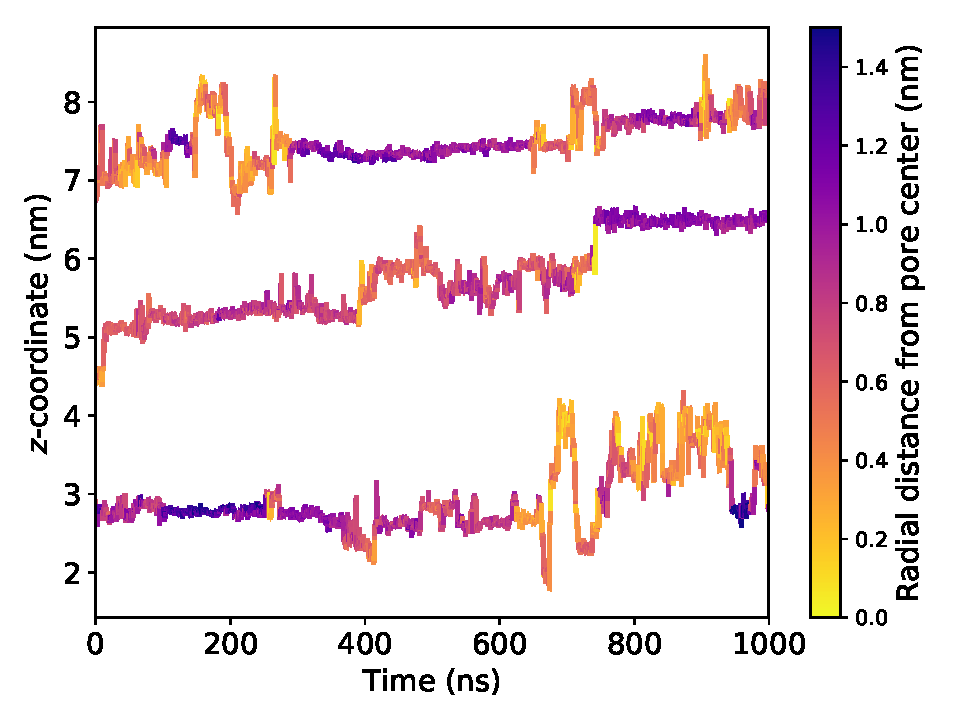
\includegraphics[width=\linewidth]{colorful_example_ztraces.pdf}
  \caption{}\label{fig:example_ztraces}
  \end{subfigure}
  \begin{subfigure}{0.49\linewidth}
  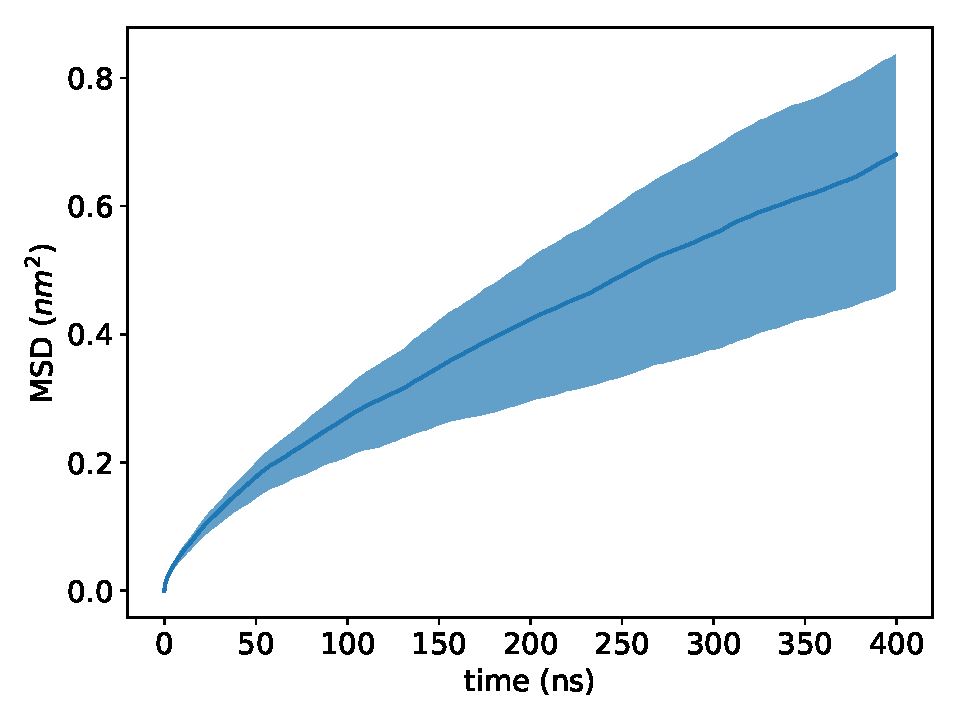
\includegraphics[width=\linewidth]{example_msd.pdf}
  \caption{}\label{fig:example_msd}
  \end{subfigure}
  \caption{All solutes show subdiffusive transport behavior inside the membrane's
  nanopores, similar to that exhibited by ethanol. (a) The $z$-coordinate trace of
  3 representative ethanol COMs shows clear periods of entrapment separated by hops.
  In general, the longest dwell times occur when solutes are situated far from the
  pore center and the hops occur when solutes are close to the pore center. (b) The
  time-averaged MSD of ethanol is sub-linear which suggests transport is governed
  by an anomalous subdiffusion process.}\label{fig:qualitative_mechanisms}

  \end{wrapfigure}
  
  Due to the crowded environment among the monomer tails, solutes generally move
  faster in the less dense pore region. Figure~\ref{fig:hop_lengths} shows that 
  this is the case for all solutes. Hops made in the pore region are on average
  59 \% larger than those made outside the pore region.
  
  However, time spent in the pore region does not necessarily result
  in a high MSD. For example, ribose spends the largest fraction of time in 
  the pore region, but has the fifth lowest hop frequency and the third 
  lowest average MSD (see Figures~\ref{fig:frac_time} and~\ref{fig:hopfreq}).
  Therefore, proximity to the pore center cannot be the sole variable that
  determines transport properties.
  
  \begin{figure}[!htb]
  \centering
  \begin{subfigure}{0.325\textwidth}
  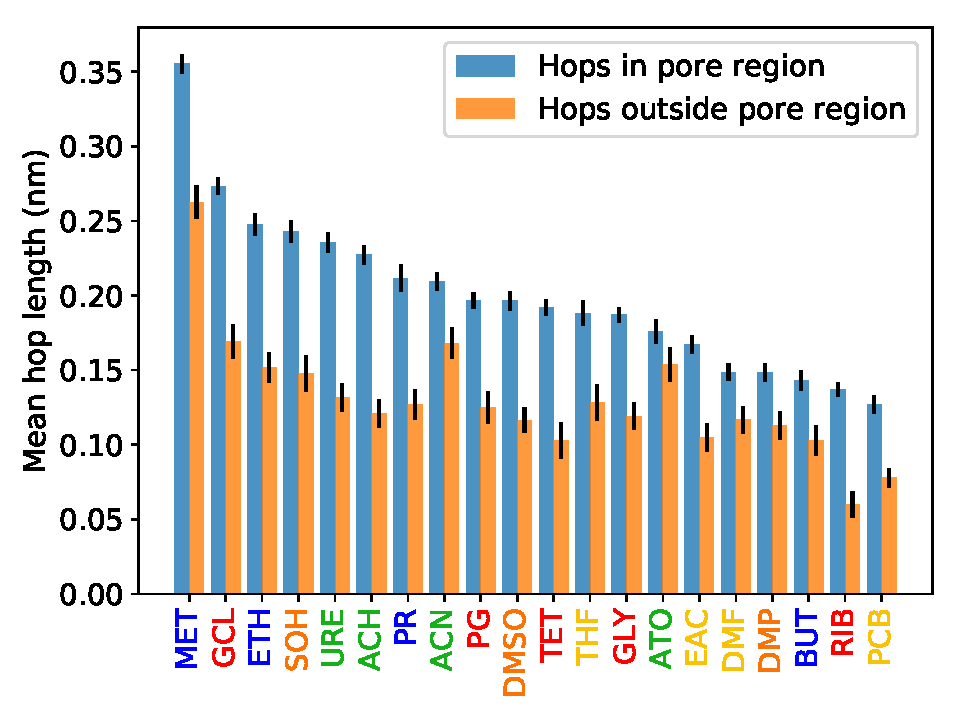
\includegraphics[width=\linewidth]{hop_length.pdf}
  \caption{}\label{fig:hop_lengths}
  \end{subfigure}
  \begin{subfigure}{0.325\textwidth}
  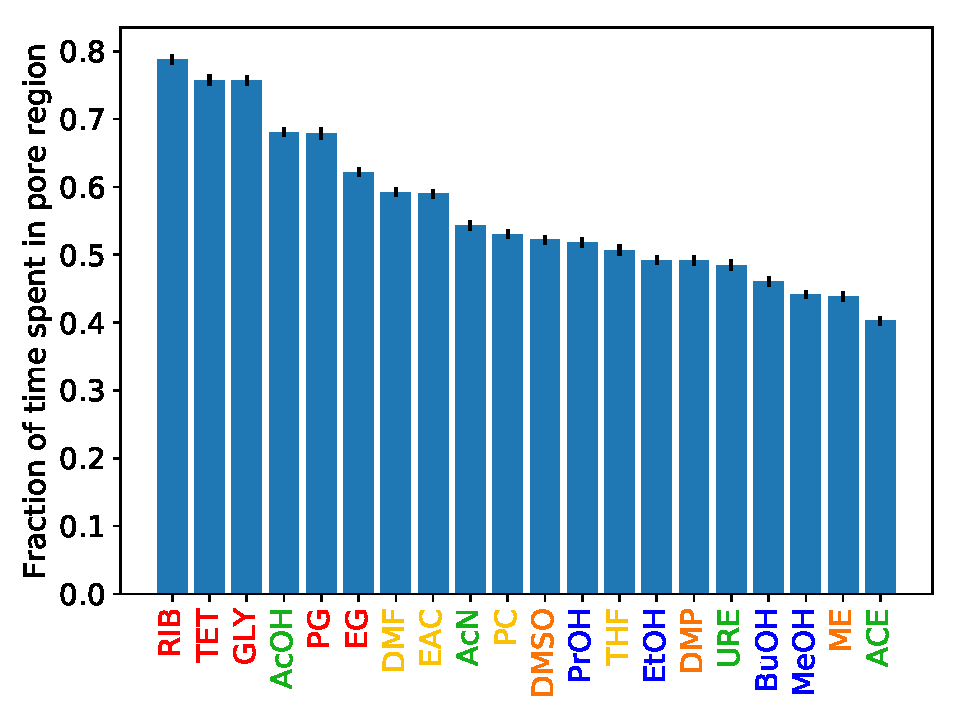
\includegraphics[width=\textwidth]{frac_time_spent.pdf}
  \caption{}\label{fig:frac_time}
  \end{subfigure}
  \begin{subfigure}{0.325\textwidth}
  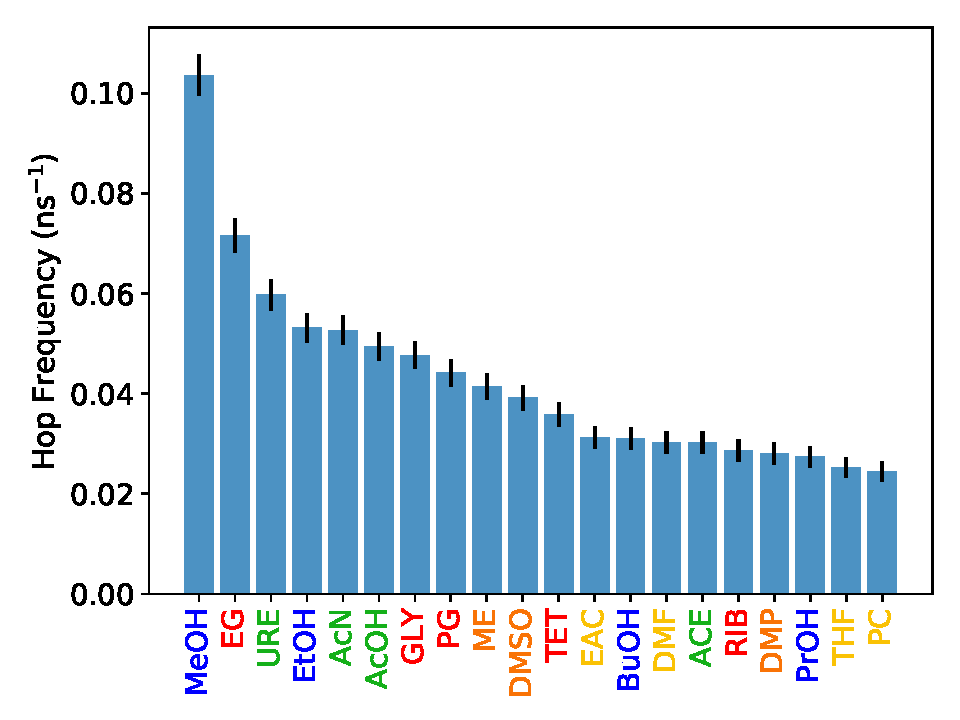
\includegraphics[width=\textwidth]{hopfreq_total.pdf}
  \caption{}\label{fig:hopfreq}
  \end{subfigure}
  \caption{(a) Hops made in the pore region of the 10 wt\% water system
  are, on average, 59 \% larger than those made outside the pore region.
  The trend in hop lengths is similar to the trend in MSDs shown in
  Figure~\ref{fig:all_msds_10wt} implying that solutes which make consistently
  larger hops have higher MSDs. The fraction of time spent by a solute in the
  pore region (b) does not necessarily lead to more frequent hopping (c). For
  example, ribose spends the largest fraction of time in the pore region, yet
  performs the the fifth lowest number of hops and third lowest MSD.}\label{fig:hops}
  \end{figure}
  
  Among the set of solutes studied, we observe three different mechanisms 
  of entrapment that are responsible for subdiffusive behavior:
  \begin{enumerate}
    \item As already demonstrated by Figures~\ref{fig:example_ztraces} and 
    Figure~\ref{fig:hop_lengths}, solutes that drift away from the pore center
    can become entangled in the monomer tails. 
    \item Many of the solutes we studied are capable of donating hydrogen bonds to
    monomer head groups and thus are prone to temporary immobilization through 
    this interaction.
    \item Because all solutes are polar, they have regions of concentrated electron
    density, modeled as partial charges, which can associate with sodium ions
    bound to monomer head groups.
  \end{enumerate}
  
  \begin{wrapfigure}{L}{0.7\textwidth}
  \centering
  \vspace{-0.35cm}
  \begin{subfigure}{0.49\linewidth}
  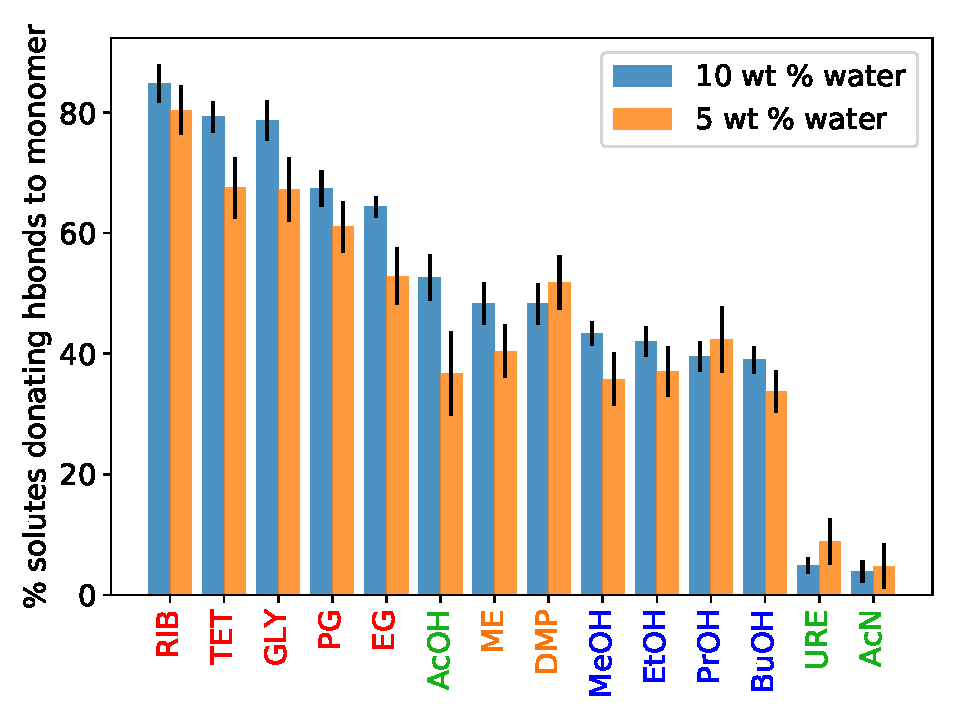
\includegraphics[width=\linewidth]{nhbonds_all.pdf}  % unique_hbonds.py
  \caption{}\label{fig:nhbonds}
  \end{subfigure}
  \begin{subfigure}{0.49\linewidth}
  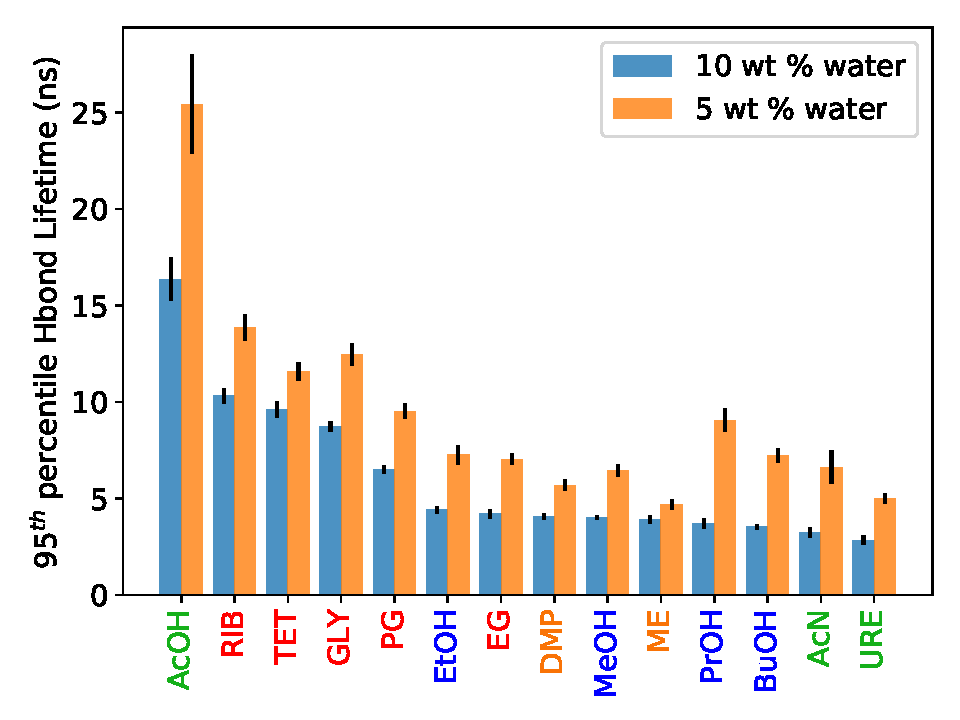
\includegraphics[width=\linewidth]{hbond_lifetime.pdf}  % hbond_dwells.py
  \caption{}\label{fig:hbond_dwells}
  \end{subfigure}
  \caption{(a) Solutes capable of donating hydrogen bonds to monomer head groups
  do so to varying degrees. The reported percentages represent unique solute-monomer
  hydrogen bonds. Individual solutes that hydrogen bond with multiple head groups
  simultaneously are only counted once. (b) The lifetime of individual hydrogen
  bonds appears correlated to the percentage of solutes involved in hydrogen bond
  interactions. Hydrogen bond lifetimes tend to be longer for solutes that
  hydrogen bond frequently. Note that solutes incapable of donating hydrogen
  bonds are omitted from this figure.}\label{fig:hbonds}
  \vspace{-0.5cm}
  \end{wrapfigure}
  
  The frequency with which solutes donate hydrogen bonds to monomer head 
  groups is related to the number of hydrogen bond donating atoms as well
  as their identity. The percentage of solutes actively participating in
  at least one hydrogen bond with a head group each frame descends as the
  number of hydroxyl groups decreases (Figure~\ref{fig:nhbonds}). Solutes
  with many hydroxyl groups, such as ribose, tetrose and glycerol, can 
  donate multiple hydrogen bonds to monomer head groups simultaneously. 
  When one hydrogen bond is broken, other hydrogen bonds work to hold the
  solute in place, which allows broken hydrogen bonds to reform. Solutes 
  containing sulfur and nitrogen atoms in place of oxygen atoms hydrogen
  bond less frequently since they are less electronegative elements.~\cite{biswal_hydrogen_2015} % citation
  The lifetime of hydrogen bonds follows nearly the same trend 
  (Figure~\ref{fig:hbond_dwells}). Hydrogen bonds of solutes that hydrogen
  bond more frequently last longer.
  
  \begin{wrapfigure}{r}{0.7\textwidth}
  \centering
  \begin{subfigure}{0.49\linewidth}
  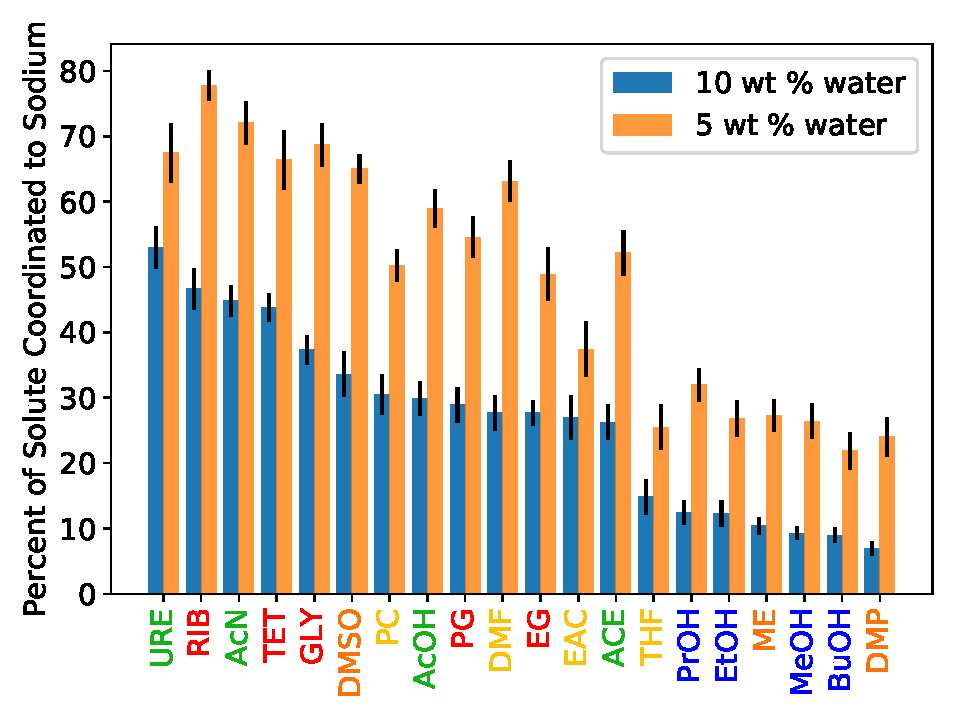
\includegraphics[width=\linewidth]{all_solutes_NA_coordination.pdf}
  \caption{}\label{fig:all_solutes_NA_coordination}
  \end{subfigure}
  \begin{subfigure}{0.49\linewidth}
  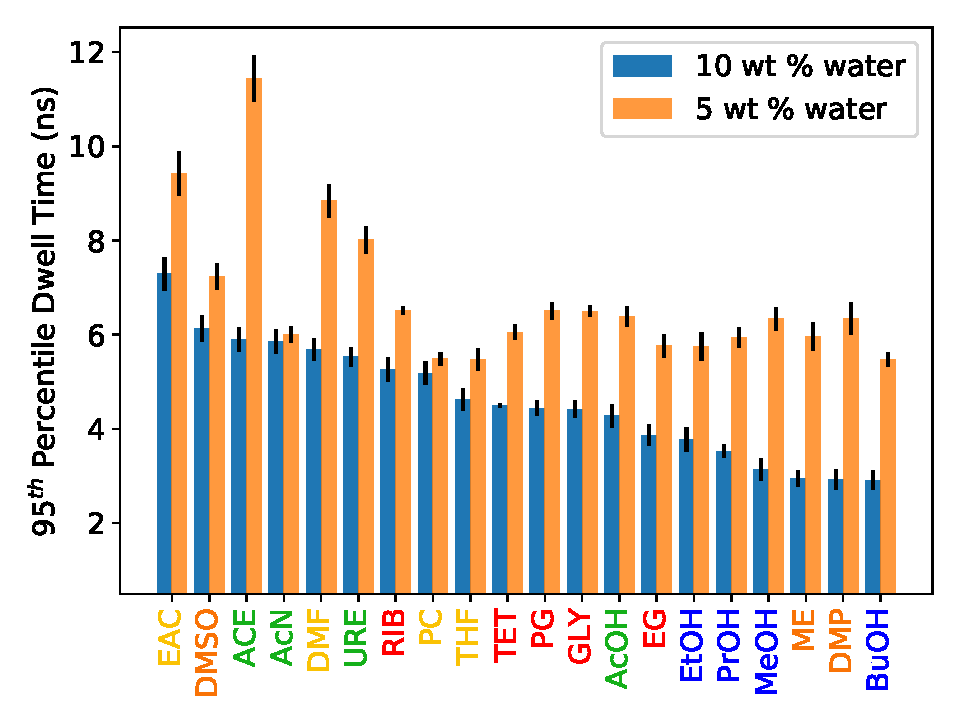
\includegraphics[width=\linewidth]{all_NA_dwells.pdf}
  \caption{}\label{fig:all_NA_dwells}
  \end{subfigure}
  \caption{(a) Solutes, especially those with carbonyl groups, spend a
  significant fraction of time coordinated to sodium ions. (b) The length
  of time a solute-sodium pairs spends associated tends to be higher for
  pairs that associate more frequently.}\label{fig:na_coordination}
  \vspace{-0.5cm}
  \end{wrapfigure}
  
  Solutes with carbonyl groups tend to associate with sodium ions most frequently.
  Nearly all of the most coordinated solutes contain a carbonyl group, except
  for DMSO which has an analogous sulfinyl group (see 
  Figure~\ref{fig:all_solutes_NA_coordination}). There is a significant drop
  in sodium ion association for solutes that do not contain carbonyl groups or
  multiple hydroxyl groups to compensate. The corresponding dwell times 
  follow a similar trend, however the dwell times of highly coordinated solutes
  with multiple hydroxyl groups are generally lower since association between
  hydroxyl groups and sodium is apparently a weaker interaction 
  (Figure~\ref{fig:all_NA_dwells}). Solutes with nitrogen atoms adjacent to 
  the carbonyl groups tend to associate with sodium ions significantly more.
  
  \begin{figure}[h!]
  \centering
  \begin{subfigure}{0.325\textwidth}
  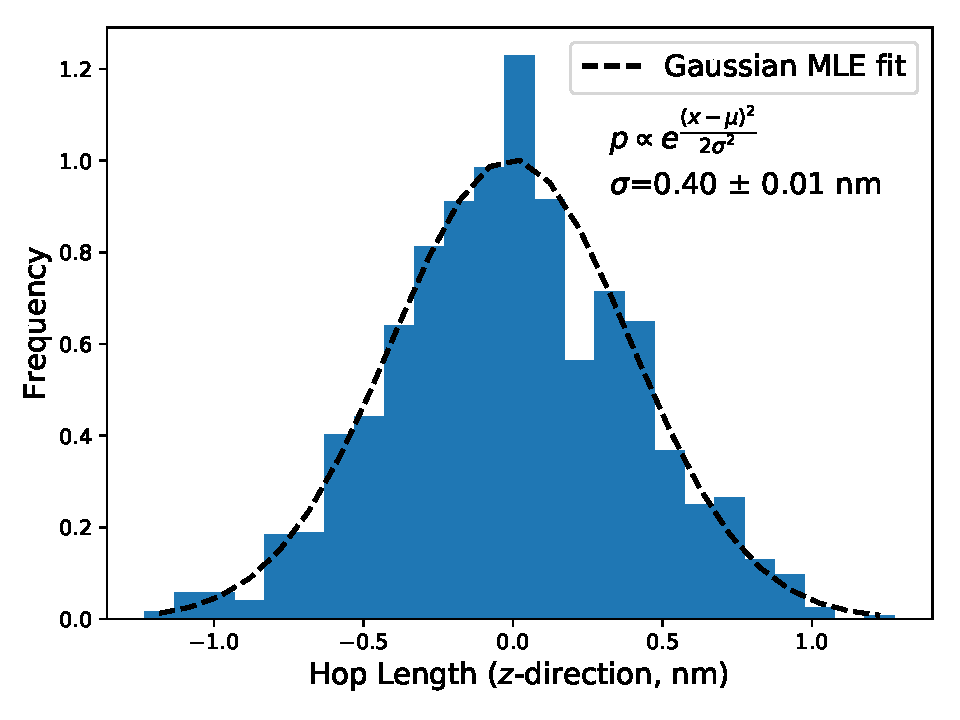
\includegraphics[width=\linewidth]{hop_distribution_GCL.pdf}
  \caption{}\label{fig:hop_dist}
  \end{subfigure}
  \begin{subfigure}{0.325\textwidth}
  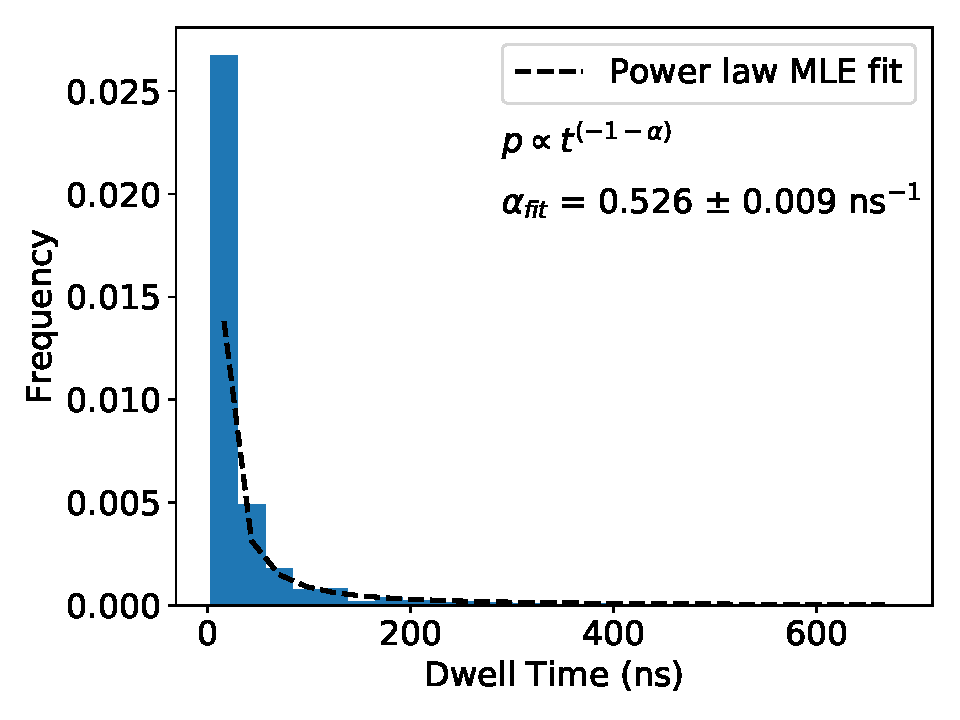
\includegraphics[width=\linewidth]{dwell_distribution_GCL.pdf}
  \caption{}\label{fig:dwell_dist}
  \end{subfigure}
  \begin{subfigure}{0.325\textwidth}
  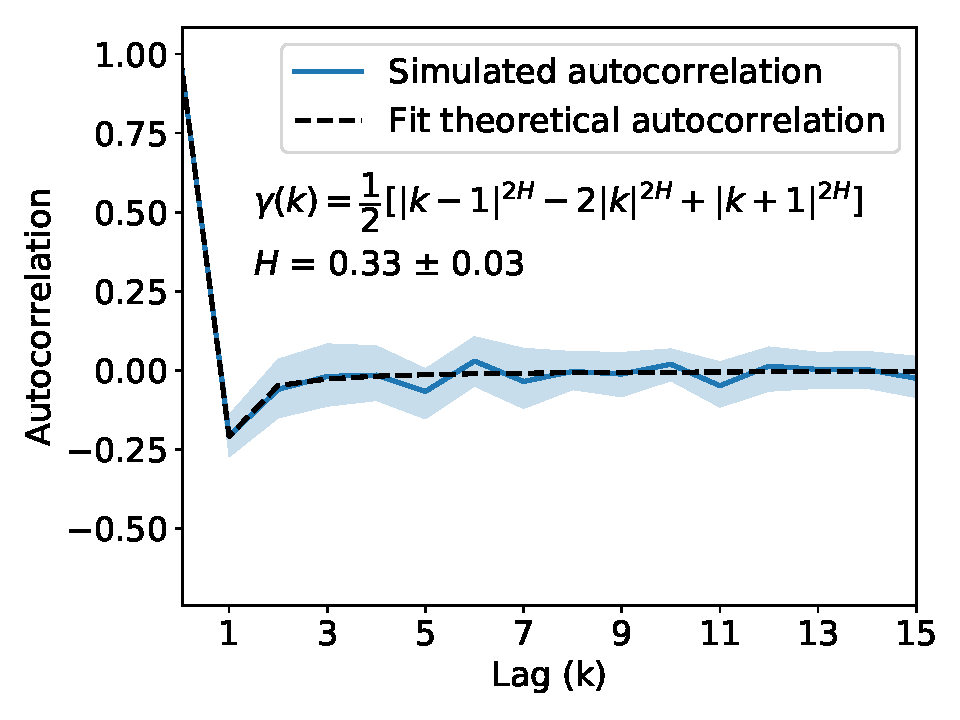
\includegraphics[width=\linewidth]{hop_acf_GCL.pdf}
  \caption{}\label{fig:hop_acf}
  \end{subfigure}
  \caption{The movement of solutes may be well-described by an sFBM process 
  which can be simulated using parameters that describe the solute's hop lengths, 
  dwell times and degree of correlation between hops. Here I use the parameters 
  derived from ethylene glycol as an example. (a) The distribution of hop
  lengths made by ethylene glycol appears Gaussian, which can be described by the
  maximum likelihood estimate (MLE) of the $\sigma$ parameter, with assumed mean, 
  $\mu$, of 0. (b) The distribution of dwell times between hops can be fit to a 
  power law whose decay is described by the MLE of the parameter $\alpha$. 
  (c) Hops are anticorrelated to their previous hop as indicated by the negative
  value at $k=1$ of the autocorrelation function, $\gamma$. The Hurst 
  parameter, $H$, is a measure of long term memory of the hops and is directly
  related to the autocorrelation function of a fractional Brownian process.}\label{fig:distributions}
  \end{figure}
  
  \noindent \textbf{\large Objective 3:} \textit{\large Create a stochastic model} (\textcolor{blue}{\textbf{In Progress}})
  
  While one can clearly learn a great deal of qualitative information about 
  mechanistic behavior on MD-accessible timescales, my work's impact would
  greatly increase if I could create a model that could predict macroscopic
  quantities such as permeability and selectivity within a reasonable degree
  of certainty. A stochastic model derived from simulation data could achieve 
  this however, there is not a well-defined procedure for this type of 
  extrapolation. Therefore, I am exploring two different approaches towards
  this end. 

  \begin{wrapfigure}{r}{0.4\textwidth}
  \centering
  \vspace{-0.6cm}
  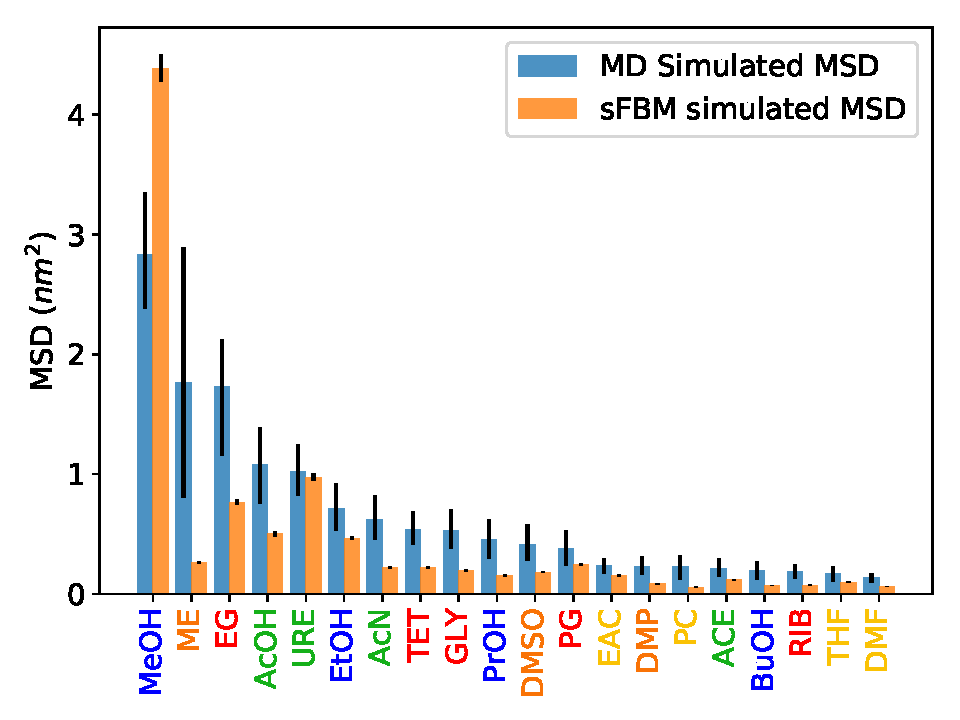
\includegraphics[width=\linewidth]{all_tamsds.pdf}
  \caption{The trends in the MSD calculated directly from MD simulations and from
  realizations of the sFBM process mostly agree, but the sFBM predictions are generally
  far too low.}\label{fig:sFBM_MSDs}
  \vspace{-0.5cm}
  \end{wrapfigure}

  \textit{Approach 1: subordinated fraction Brownian motion}: My first route 
  towards a stochastic model is to simulate realizations of a subordinated 
  fractional Brownian motion (sFBM) process based on parameters extracted 
  from solute time series. As demonstrated by the example in 
  Figures~\ref{fig:hop_dist} and~\ref{fig:dwell_dist}, hop length 
  distributions in the $z$-direction appear Gaussian while the distribution
  of dwell times between hops appears to be distributed according to a power
  law. Alone, these distributions characterize a continuous time random walk
  (CTRW), which is a subdiffusive process where particles hop a random distance
  in a random direction and stay there for a random period of time.~\cite{meroz_toolbox_2015}.
  Unlike a CTRW, the hops in the system I study appear anti-correlated to 
  their previous hop as demonstrated by the autocorrelation function in 
  Figure~\ref{fig:hop_acf}. A CTRW with anticorrelated hops is well-described
  by an sFBM process.~\cite{meroz_subdiffusion_2010}

%  \begin{wrapfigure}{l}{0.6\textwidth}
%  \centering
%  \vspace{-0.5cm}
%  \begin{subfigure}{0.49\linewidth}
%  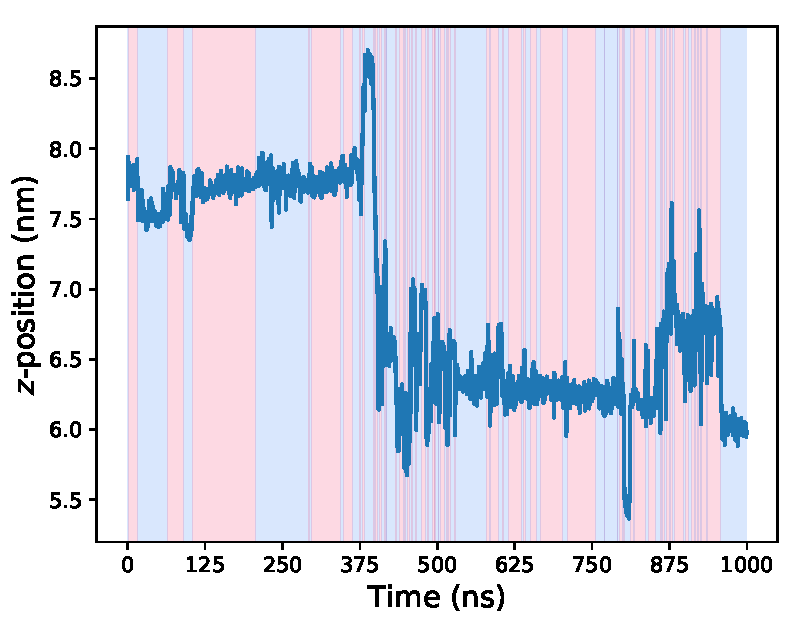
\includegraphics[width=\linewidth]{breakpoints.pdf}
%  \caption{}\label{fig:breakpoints}
%  \end{subfigure}
%  \begin{subfigure}{0.49\linewidth}
%  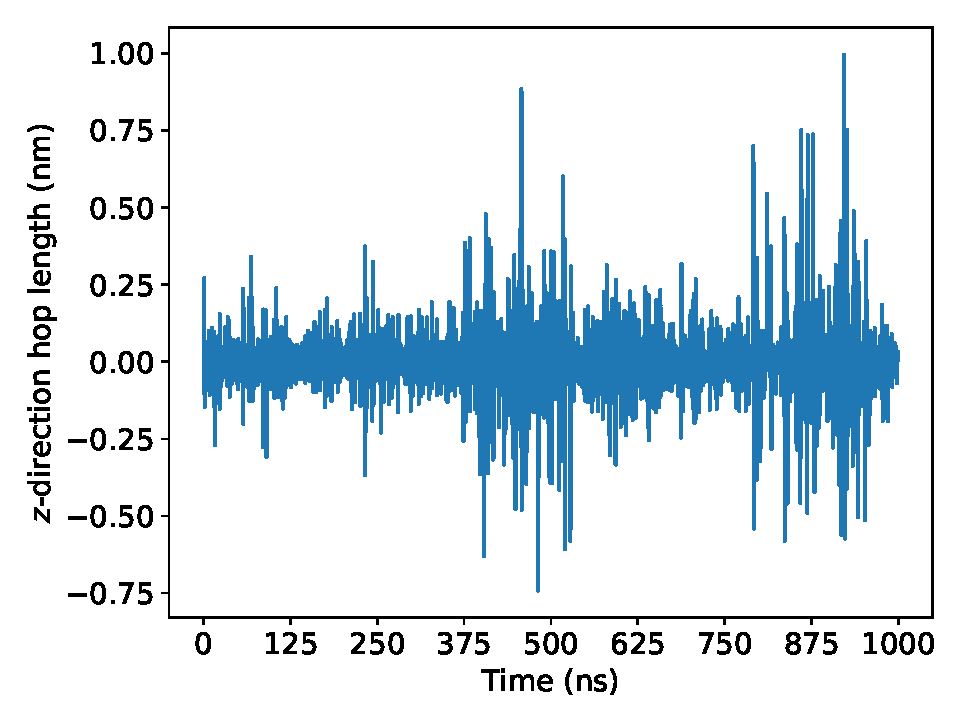
\includegraphics[width=\linewidth]{first_order_difference.pdf}
%  \caption{}\label{fig:first_order_difference}
%  \end{subfigure}
%  \begin{subfigure}{0.49\linewidth}
%  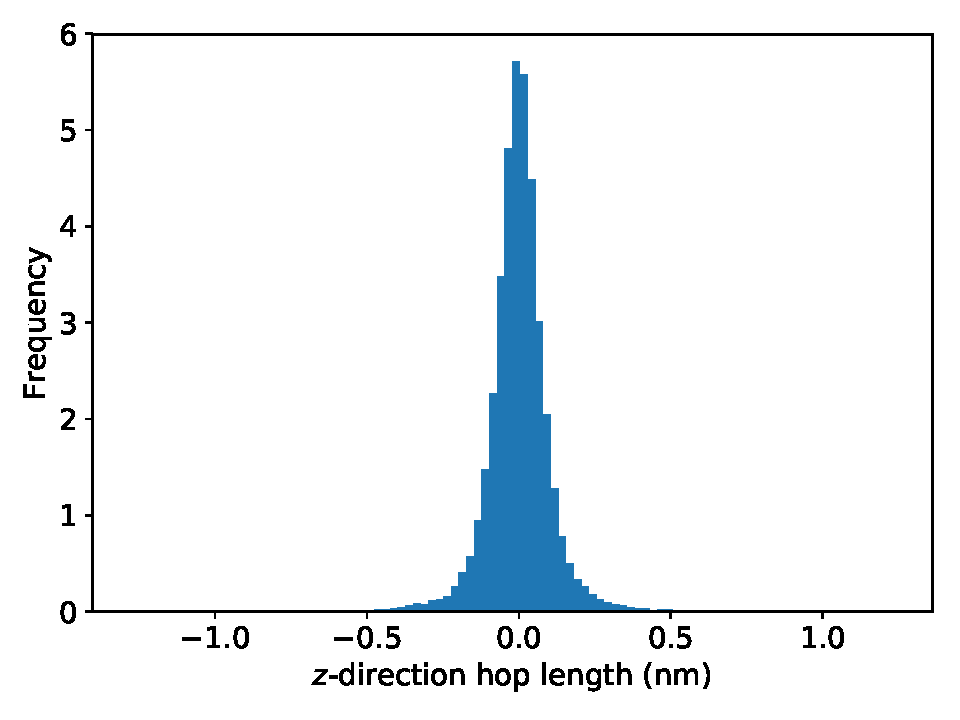
\includegraphics[width=\linewidth]{hop_density.pdf}
%  \caption{}\label{fig:hop_density}
%  \end{subfigure}
%  \begin{subfigure}{0.49\linewidth}
%  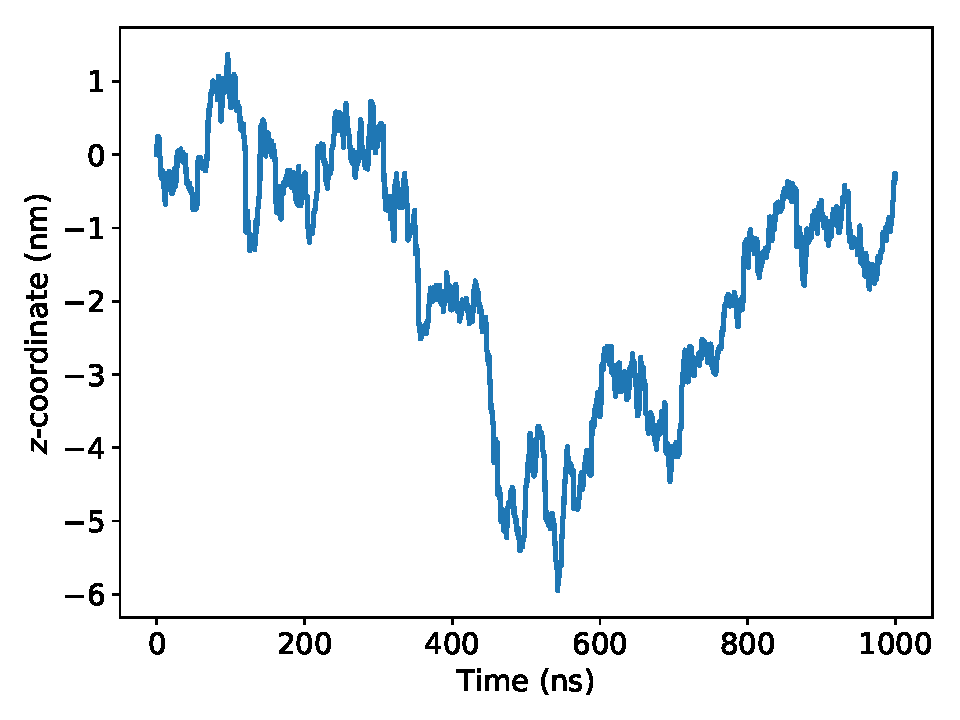
\includegraphics[width=\linewidth]{naive_density_forecast.pdf}
%  \caption{}\label{fig:naive_density_forecast}
%  \end{subfigure}
%  \caption{In contrast to our first approach which relies on accurate 
%  detection of hops, density forecasting uses all of the time series 
%  information at our disposal. (a) Our first approach identifies hops 
%  based on breakpoints, indicated by color transitions. All information 
%  is lost between breakpoints. (b) Instead we can calculate hop lengths
%  between each time step and (c) compile them into a single probability 
%  density. (d) As a first approximation, one can simulate time series
%  by randomly drawing from the distribution in (c).}\label{fig:density_forecast}
%  \vspace{-1.5cm}
%  \end{wrapfigure}  
  
  Solute MSDs calculated based on realizations of an sFBM process mostly
  preserve the trends in MSD calculated directly from MD simulations (see
  Figure~\ref{fig:sFBM_MSDs}), but the predictions are generally too low. 
  For each solute, I used the parameters described in Figure~\ref{fig:distributions}
  to generate $1e4$ realizations of an sFBM process, each with the same
  length as the MD simulations (1000 ns) so that I could make a direct 
  comparison between their MSDs. While the sFBM MSD prediction for methanol
  is too high, the rest are on average only 46\% of the MD calculated MSD
  values. 
  
%  \begin{wrapfigure}{r}{0.4\textwidth}
%  \centering
%  \vspace{-0.5cm}
%  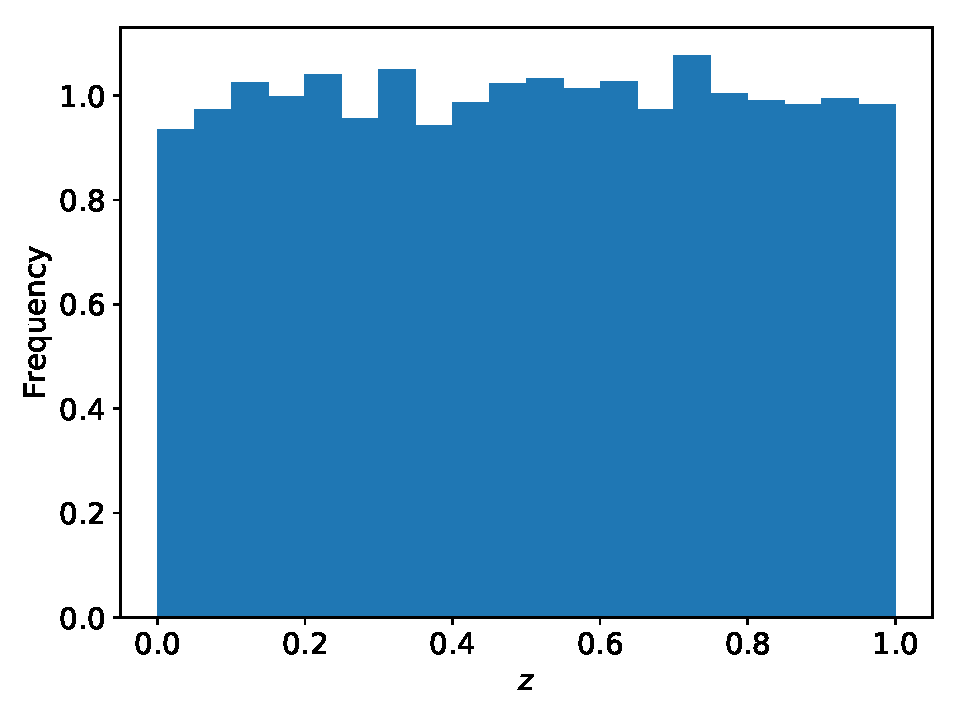
\includegraphics[width=\linewidth]{z_histogram.pdf}
%  \caption{The histogram of $z$ values coming from $z_t$ calculated with 
%  Equation~\ref{eqn:pit} appears uniform meaning $p(h)$ is well-sampled 
%  by the out-sample data.}\label{fig:z_histogram}
%  \vspace{-1cm}
%  \end{wrapfigure}
  
  \begin{wrapfigure}{l}{0.4\textwidth}
  \centering
  \vspace{-0.5cm}
  \begin{subfigure}{\linewidth}
  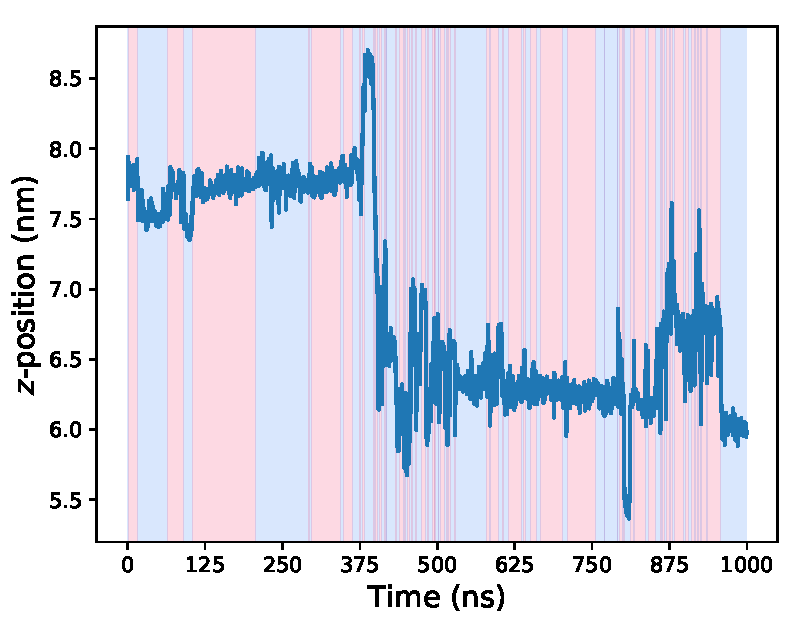
\includegraphics[width=\linewidth]{breakpoints.pdf}
  \caption{}\label{fig:breakpoints}
  \end{subfigure}
  \caption{In order to generate the parameters used in our first approach,
  I identified hops based on change points in the time series, indicated by
  color transitions. In addition to errors in change point detection, all 
  information between change points is lost.}\label{fig:ruptures}
  \vspace{-.5cm}
  \end{wrapfigure}  
  
  This approach might be improved by incorporating radial dependence into
  the three sFBM parameters described in Figure~\ref{fig:distributions}. 
  In Figure~\ref{fig:hop_lengths}, we showed that hops by solutes situated 
  inside the pores are 59\% larger than hops by solutes in the tails, which 
  leads to two distinct values of $\sigma$. Similarly, we can determine 
  radially dependent values of $\alpha$ and $H$. 
  
  A simple two state model, in pore versus out of pore, may be sufficient to 
  fully incorporate radially dependent effects. Based on the fraction of time 
  spent in the pore region (Figure~\ref{fig:frac_time}), we can determine
  the appropriate balance of each type of parameter to use when simulating sFBM
  realizations. We would also need some kind of switching frequency, or dwell
  time in each region since it does not make physical sense for a solute to 
  enter and exit the pore region every other time step.
  
  If the two state model proves insufficient, I can add increasing levels of
  complexity. For example, I might make the radial dependence a continuous 
  function, or I could assign parameters that are dependent on the type of
  trapping mechanism affecting the solute.
  
  It is important to note that this first approach throws out a significant fraction
  of the data. In order to construct distributions of hop lengths and dwell 
  times with my first approach, I needed to locate precise time points at which
  hops occurred. We achieved this using an off-line change point detection algorithm implemented
  in the python package \texttt{ruptures}.~\cite{truong_review_2018} The 
  algorithm does a decent job of identifying hops, but still loses information
  as demonstrated in Figure~\ref{fig:breakpoints}. 

  \textit{Approach 2: Markov Switching Models}: Instead of limiting my 
  analysis to 3 fitting parameters ($\alpha$, $\sigma$ and $H$), my second
  approach uses all of the available data in order to classify sequences
  of time series behavior into distinct states. In 
  Figure~\ref{fig:markov_states_timeseries}, for demonstrative purposes,
  I've identified 3 potential states defined by the solute's behavior 
  during the time bounded by each box. Once we've identified states, we 
  can use our data to define a matrix of probabilities describing switches
  between states, following a Markovian framework (see Figure~\ref{fig:markov}).~\cite{howard_dynamic_1960}
  
  \begin{figure}
  \centering
  \vspace{-0.5cm}
  \begin{subfigure}{0.725\linewidth}
  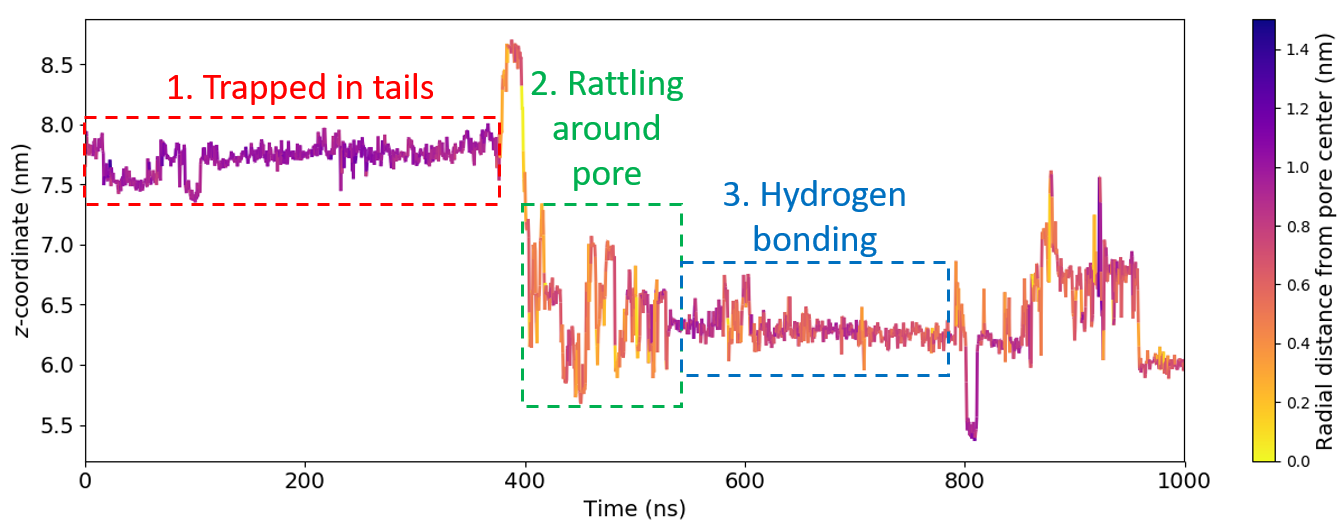
\includegraphics[width=\linewidth]{markov_states_timeseries.png}
  \caption{}\label{fig:markov_states_timeseries}
  \end{subfigure}
  \begin{subfigure}{0.25\linewidth}
  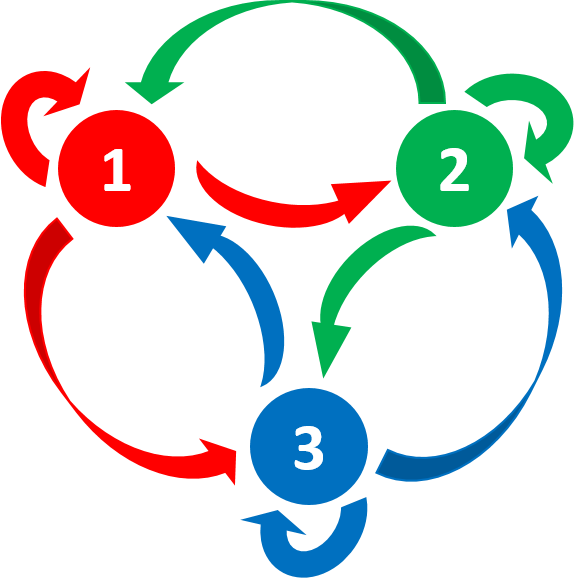
\includegraphics[width=\linewidth]{markov.png}
  \caption{}\label{fig:markov}
  \end{subfigure}
  \caption{Using my second approach, I will be able to classify the behavior
  of solutes into distinct states. (a) As an example, I've come up with three
  potential states based on the time series pictured above. State 1: solutes
  far from the pore region are trapped in the tails leading to restricted 
  motion. State 2: unbound solutes within the pores make large and frequent
  movements. State 3: solutes donating hydrogen bonds to monomer head groups
  tend to stay in place. (b) There is a probability associated with each
  transition between states, represented by the arrows above. For example, following
  the red arrows, there are probabilities associated with going from State 1 to
  State 2, from State 1 to State 3 and from State 1 back to State 1.
  }\label{fig:markov_states}
  \vspace{-.5cm}
  \end{figure}
  
  I will use the Kalman filter algorithm in order to identify distinct states
  in solute time series and simultaneously describe the dynamics of each state.~\cite{kalman_new_1960}
  In general, the Kalman filter can attempt to linearly project subsequent 
  steps in a time series based on its past values. The error in each prediction
  is stored sequentially. Regions of the time series associated with the 
  largest prediction uncertainties can be used as an indication of a state change.
  Using a non-parametric Bayesian approach to identify states, I will not need to 
  pre-define the number of states which will allow the data to drive the
  model's complexity.~\cite{lee_unraveling_2017} A convenient byproduct of the Kalman
  filter are maximum likelihood estimates for parameters which describe the times
  series in terms of an autoregressive moving average (ARMA) process:~\cite{hamilton_time_1994}
  \begin{equation}
  Y_t = c + \phi_1 Y_{t-1} + \phi_2 Y_{t-2} + \cdot\cdot\cdot + \phi_p Y_{t-p} + \epsilon_t + \theta_1\epsilon_{t-1} + \theta_2\epsilon_{t-2} + \cdot\cdot\cdot + \theta_q\epsilon_{t-q}
  \label{eqn:arma}
  \end{equation}
  where $Y_t$ represents the time series value at time $t$, $\epsilon$ is a white noise
  parameter and $\phi$ and $\theta$ are coefficients determined by the Kalman filter. 
  With knowledge of the transition probabilities and the dynamic behavior of each
  state described by Equation~\ref{eqn:arma}, I can forecast solute time series orders of 
  magnitude longer than with molecular simulations.
  
%  Density forecasting can provide
%  predictions based on properties of a time series without any knowledge
%  of the physical interactions leading to those properties. 
  
%  \begin{wrapfigure}{l}{0.6\textwidth}
%  \centering
%  \vspace{-0.75cm}
%  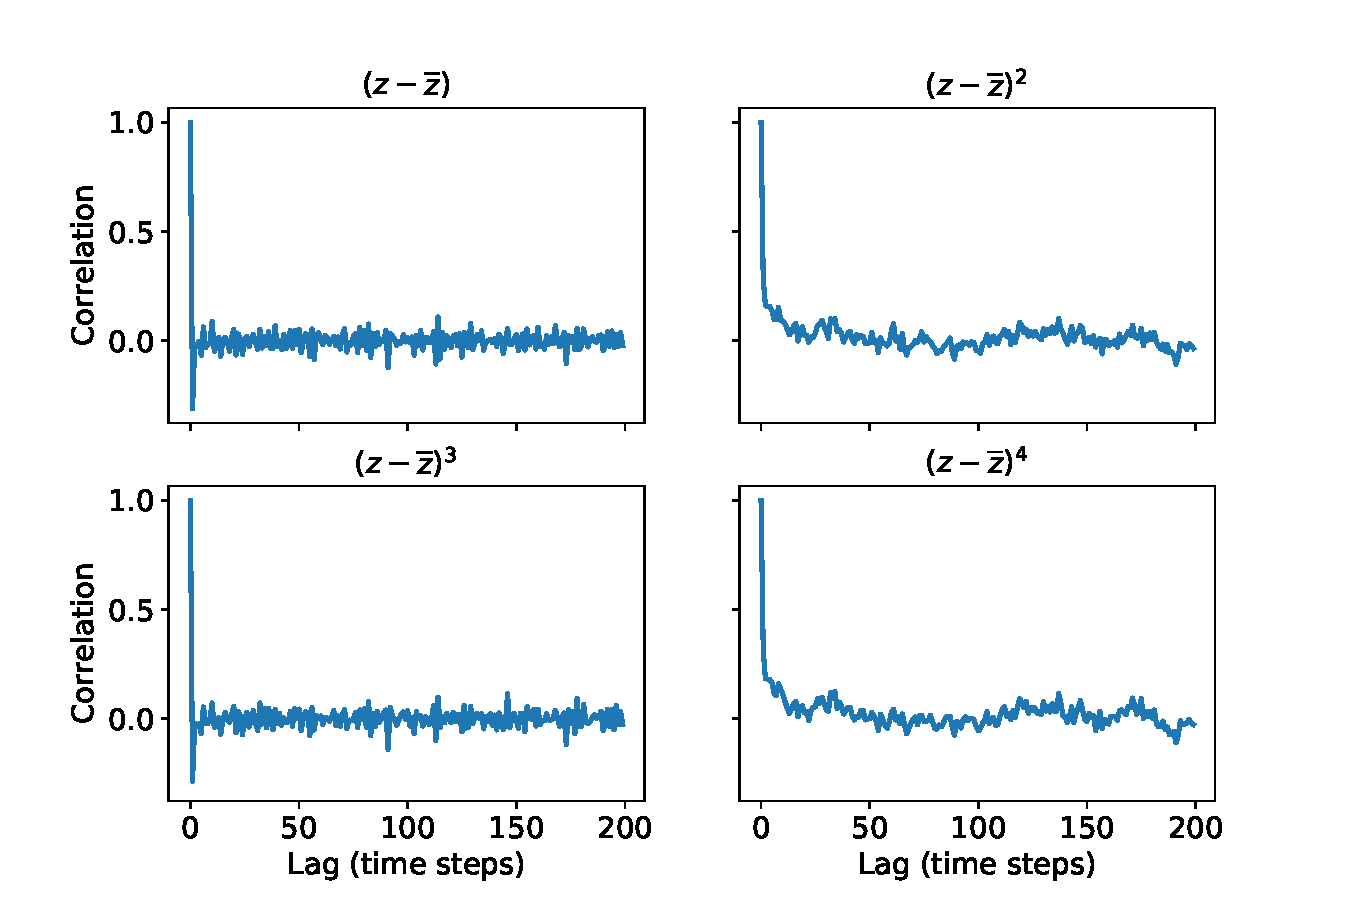
\includegraphics[width=\linewidth]{correlograms.pdf}
%  \caption{Correlograms of $z_t$ reveal dependence for all 4 powers of 
%  $(z - \overline{z})$.}\label{fig:correlograms}
%  \vspace{-0.5cm}
%  \end{wrapfigure}
  
%With density forecasting, one can instead 
%  compile the hop length and magnitude between each time step 
%  (Figure~\ref{fig:first_order_difference}) into a probability density
%  like that shown in Figure~\ref{fig:hop_density}. As a first attempt, 
%  one could randomly draw from this distribution in order to construct
%  a time series like that shown in Figure~\ref{fig:naive_density_forecast}.
  
%  One can test how well a time series of hop lengths, $h_t$, is described by the 
%  hop density, $p(h)$, in Figure~\ref{fig:hop_density} using the probability
%  integral transform:~\cite{diebold_evaluating_1998}
%  \begin{equation}
%  z_t = \int_{-\infty}^{h_t} p(u) du
%  \label{eqn:pit}
%  \end{equation}
%  Generally, one uses the first half of a time series, or in-sample data, to
%  create $p(h)$ and applies Equation~\ref{eqn:pit} to the second half of
%  the time series, or out-sample data. If the distribution of $z_t$ values
%  is uniform, then the cumulative distribution function of $p(h)$ has been
%  sampled uniformly by the out-sample data and there is evidence that the 
%  time series is well-described by $p(h)$. Using the out-sample data from 
%  Figure~\ref{fig:density_forecast}, we observe a uniform distribution of
%  $z_t$ values (Figure~\ref{fig:z_histogram}).
  
%  However, it is also necessary to look for correlations in $z_t$. Diebold
%  et al. found that examination of the correlograms of $(z - \overline{z})$,
%  $(z - \overline{z})^2$, $(z - \overline{z})^3$ and $(z - \overline{z})^4$,
%  which represent dependence of the mean, variance, skewness and kurtosis 
%  respectively, are adequate to identify potentially sophisticated and 
%  nonlinear forms of past dependence.~\cite{diebold_evaluating_1998} Continuing
%  with our example above, the correlograms of $z_t$ shown in Figure~\ref{fig:correlograms} 
%  exhibit serial dependence for all powers of $(z - \overline{z})$. Our 
%  time series exhibits dependence on its past values, a feature that was 
%  not included in the forecast shown in Figure~\ref{fig:naive_density_forecast}.
  %This likely explains the qualitative difference in the time series of 
  %Figure~\ref{fig:breakpoints} versus~\ref{fig:naive_density_forecast}.
  
%  Going forward, I will need to incorporate previous dependence in the 
%  form of a conditional density forecast with the form $p(h|\Omega_t)$ where
%  $\Omega_t$ incorporates past hop lengths and radial distances from
%  the pore center. These types of autoregressive models have been widely
%  studied in the context of economics, but are still well-suited for 
%  application to solute transport.~\cite{hamilton_time_1994}
  
  \noindent \textbf{\large Objective 4:} \textit{\large Apply analyses to 
  Q\textsubscript{I} phase} (\textcolor{blue}{\textbf{In Progress}})
  
  Paralleling my work on the H\textsubscript{II} phase, my first task towards
  this objective was to build a suitable unit cell representation of the 
  Q\textsubscript{I} phase. Unfortunately, the true space group of the 
  Q\textsubscript{I} phase that we are studying is unknown. Experimental 
  diffraction has narrowed down the possible bicontinuous cubic 
  configurations to the Ia3d and Pn3m space groups.~\cite{pindzola_cross-linked_2003}
  Therefore, we will build both types of unit cells and search for clues that
  can be used to differentiate them experimentally.
  
  \begin{wrapfigure}{l}{0.6\textwidth}
  \centering
  \vspace{-0.5cm}
  \begin{subfigure}{0.49\linewidth}
  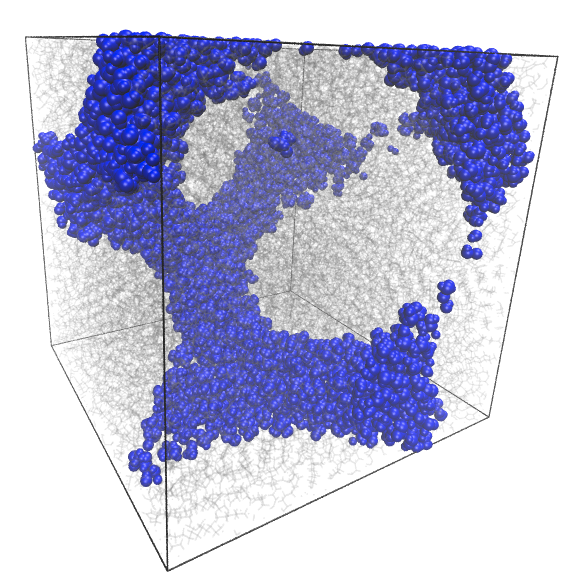
\includegraphics[width=\linewidth]{gyroid.png}
  \caption{}\label{fig:Ia3d}
  \end{subfigure}
  \begin{subfigure}{0.49\linewidth}
  \includegraphics[width=\linewidth]{schwarz.png}
  \caption{}\label{fig:pn3m}
  \end{subfigure}
  \caption{I developed a procedure capable of building both (a) Ia3d and (b) Pn3m
  unit cells from arbitrary monomers with controllable pore size. The blue
  glycerol molecules highlight the aqeuous region where transport occurs.}\label{fig:q1_unitcells}
  \vspace{-0.5cm}
  \end{wrapfigure}
  
  I have developed a procedure that can build both Ia3d and Pn3m unit cells.
  To our knowledge, nobody has ever built an atomistic molecular model of 
  a bicontinuous cubic phase system. Some systems have been created by 
  allowing coarse grained representations to self-assemble over long 
  timescales.~\cite{mondal_self-assembly_2013} However, self-assembly
  can be a long process, especially for fully atomistic systems, where it
  might take multiple orders of magnitude longer than what we can 
  reasonably simulate. Instead, I use analytical equations that describe
  the surface of these systems in order to place monomers into a unit cell.~\cite{benedicto_bicontinuous_1997}
  Monomers are placed perpendicular to the surface in random locations 
  that don't overlap. One can control the pore size by translating monomers
  perpendicular to the surface at the point where they are attached.
  
  First, I will study the structure of the Q\textsubscript{I} phase using
  methodology similar to that used for the H\textsubscript{II} phase 
  I will attempt to identify one of the space groups as the most likely
  experimental configuration based on simulated XRD signatures, although
  this might not work due to the known similarity of Ia3d and Pn3m XRD 
  patterns.
  
  Then I will study transport of solutes within these atomistic unit cells, 
  adapting the same analyses used in Objectives 2--3. The primary 
  challenge will be adapting my techniques to the more complex pore geometry
  of the Q\textsubscript{I} phase, however I expect that the main conclusions
  will not deviate far from those of the H\textsubscript{II} phase since
  the chemical environments within the nanopores are qualitatively similar. 
  
  The experimental performance of Q\textsubscript{I} phase membranes has been
  studied far more extensively than that of the H\textsubscript{II} phase. 
  Therefore, I may be able to identify which space group is correct if
  one system exhibits experimentally inconsistent transport properties and one
  does not. I can attempt to replicate the trends in the results of the separation
  studies performed by Dischinger et al.~\cite{dischinger_application_2017} If
  I can match the experimental trends, then there is a good chance that I can
  use my molecular model to offer an explanation for the complex behavior described
  in their work (see first paragraph of Section~\ref{section:objectives}).

  %MRS2: emphasize comparison to experiments more here, based on what they have done, and what they will do; outline how you will compare to those experiments.

%  \noindent \textbf{\large Objective 5} \textit{\large Create a well-documented python package} (\textcolor{blue}{\textbf{In Progress}})
%  
%  Python scripts used to simulate X-ray diffraction patterns are available in the following
%  GitHub repository: \url{https://github.com/joeyelk/MD-Structure-Factor}. Documentation
%  is forthcoming. 
%  
%  Python scripts used to conduct all other post-simulation trajectory analysis are 
%  also available on GitHub: \url{https://github.com/shirtsgroup/LLC_Membranes}. 
%  Documentation is a work in progress. It is available for viewing in its 
%  current state at \url{https://llc-membranes.readthedocs.io/en/latest/}.

  \section{Timeline for Completion of Objectives}\label{section:timeline}

  A schematic of the estimated timeline that I plan to follow for the 
  completion of tasks pertinent to finishing all objectives is given 
  in Table~\ref{table:timeline}. Ideally, each task will become a 
  published manuscript. I will run simulations required to 
  study the structure of the bicontinuous cubic phase in
  parallel with the continued development of my stochastic model of 
  transport in the H\textsubscript{II} phase. Simulations and analysis
  required for Q\textsubscript{I} phase solute transport studies analogous
  to those of Objective 2 will be carried out throughout Fall 2019. 
  Application of a stochastic model to the Q\textsubscript{I} phase will
  be finished by May 2020, just before I defend my dissertation.

  \begin{center}  
  \begin{table}[!htb]
	\renewcommand\arraystretch{1.4}\arrayrulecolor{LightSteelBlue3}
	\captionsetup{singlelinecheck=false, font=blue, labelfont=sc, labelsep=quad}
	\caption{Estimated Timeline for Completion of Objectives}\vskip -1.5ex
	\begin{tabular}{@{\,}r <{\hskip 2pt} !{\foo} >{\raggedright\arraybackslash}p{8cm}}
	\toprule
	\addlinespace[1.5ex]
	August 2019 & Complete Stochastic Model for H\textsubscript{II} phase \\
	September 2019 & Finalize Q\textsubscript{I} phase structure \\
    January 2020 & Finish transport study of Q\textsubscript{I} phase \\
    April 2020 & Finish application of stochastic model to Q\textsubscript{I} phase \\
    May 2020 & PhD Defense \\
	\end{tabular}
	\label{table:timeline}
  \end{table}
  \end{center}
  \vspace{-2cm}
  
  \section{Resource Requirements}\label{section:resources}
  
  The remainder of our work will require the use of high performance computing (HPC)
  resources. We will continue using Bridges, an XSEDE resource as well as Summit, a
  supercomputer located at CU Boulder.
  
  \section{Safety Considerations}\label{section:safety}
  
  Although my work is confined to computer work in an office space, there are 
  associated health risks that I must mitigate. Proper ergonomics ensure 
  maximum comfort and help me to work efficiently. Sitting up straight and
  having proper back support are necessary to relieve pressure on the discs
  of my vertebrae. My monitors are positioned an arm's length directly in 
  front of me with the tops of the monitors at eye level in order to reduce
  head, neck and eye strain. Finally, I take frequent breaks and go for 
  walks around the building.

  \newpage
  \bibliographystyle{ieeetr}
  \bibliography{comps}

\end{document}
